\documentclass{tADR2e}

\usepackage{epstopdf}% To incorporate .eps illustrations using PDFLaTeX, etc.
\usepackage{subfigure}% Support for small, `sub' figures and tables
\usepackage{multicol}
\usepackage{multirow}
\usepackage{flushend}
\usepackage{collcell}
\usepackage{booktabs}
\usepackage[hidelinks]{hyperref}

\newcolumntype{x}[1]{>{\raggedleft\hspace{0pt}}p{#1}}
\newcommand{\ignore}[1]{}

\begin{document}

\jvol{31} \jnum{5} \jyear{2017} \jmonth{March}

\articletype{FULL PAPER}




\title{Context-Aware Robot Navigation using Interactively-Built Semantic Maps}

\author{
\name{Akansel Cosgun$^\ast$,\thanks{$^\ast$Corresponding author. Email: akansel.cosgun@gmail.com}
Alexander J. B. Trevor and Henrik I. Christensen}
\affil{Institute for Robotics and Intelligent Machines (IRIM), Georgia Institute of Technology, USA}
\received{v1.0 released May 2016}
}

\maketitle

\begin{abstract}
We discuss the process of building semantic maps, how to interactively label entities in it, and use them to enable new navigation behaviors for specific scenarios. We utilize planar surfaces such as walls and tables, and static objects such as door signs as features to our semantic mapping approach. Users can interactively annotate these features by having the robot follow him/her, entering the label through a mobile app and performing a pointing gesture toward the landmark of interest. These landmarks can later be used to generate context-aware motions. Our pointing gesture approach can reliably estimate the target object using human joint positions and detect ambiguous gestures with probabilistic modeling. Our person following method attempts to maximize future utility by searching future actions, assuming constant velocity model for the human. We describe a simple method to extract metric goals from a semantic map landmark and present a human aware path planner that considers the personal spaces of people to generate socially-aware paths. Finally, we demonstrate context-awareness for person following in two scenarios: interactive labeling and door passing. We believe as the sensing technology improves and maps with richer semantic information becomes commonplace, it would create new opportunities for intelligent navigation algorithms.
\end{abstract}

\begin{keywords}
human-robot interaction; robot navigation; semantic mapping; 
\end{keywords}


\section{Introduction}

Perhaps the most fundamental capability for a mobile robot is navigating from one location to another. Advances in mapping, localization and path planning research in the past decades made indoor navigation a commodity for mobile robots. Robots keep a representation of its environment to enable navigation behaviors, and this representation is usually in the form of a discrete \textit{metric map}, where each grid cells represent whether that position is occupied with an obstacle or not. Mobile robots that use such a map can accept navigation goals in metric coordinates, however exact coordinates may not be the most intuitive way to communicate goals for human users. Robots that navigate in human environments will need to accept human-friendly navigation goals. A map for such robots should facilitate establishment of a \textit{common ground} between the robot and its user and enable referencing to the same spatial elements. This is only possible with a richer map representation that includes \textit{semantic} information. In particular, if the humans and robots need to communicate over navigation goals that involve objects, landmarks or rooms, a map should include information about these.

Path planing for mobile robots has traditionally been considered a shortest-path problem. While this leads to sound solutions and collision-free paths, this approach is not be suitable to human environments. With a richer representation of the environment, robots would have the tools to have context-awareness for navigation. By context awareness, the mean two separate concepts: Leveraging semantic maps and human-aware robot navigation. The context of which room the robot is in, what the task is, and what objects are around could be useful for navigation. Tracking people can also enhance navigation behaviors, as the robot respects people's personal spaces and obey social norms.

In this paper, we investigate how to create a semantic map, enable humans to label the elements of the semantic map, and how the semantic map can be used to enable context-awareness in navigation. Our semantic mapping approach involves using planar surfaces such as walls and tables and static objects such as door signs for mapping. We designed an interaction pattern that enables a user to label landmarks in the semantic map, while the robot is following him/her. A user first enters a labeling request using a mobile app, then physically points at the landmark. We present a person following algorithm that aims to keep a fixed distance to the user. We also present a probabilistic model to estimate the pointing target and if there is ambiguity in determining the target. The user-annotated landmark could then be used as a navigation goal. Our path planner considers personal spaces of people and their reactions to the robot's future motions. Our approach to context-awareness is to use doors and planar surfaces to improve the person following behavior.

The main contributions of this paper are: (a) a mapping system to create semantic maps from stationary objects and planar surfaces, (a) a method for a human to take a mobile robot on a tour and interactively attach labels to the landmarks in the semantic map, (c) perception module to estimate the target of a pointing gesture, (d) a path planning algorithm that generates socially aware paths and (e) demonstration of context-awareness for person following.

The rest of this paper is organized as follows: A literature survey of related works is given in Section \ref{sec:related_works}, followed by our semantic mapping approach in Section \ref{sec:slam_and_semantic_mapping}. Section \ref{sec:interactive_map_labeling} describes how users interactively label semantic elements, as well as components that enable labeling: person following and pointing gestures. In Section \ref{sec:evaluation}, we evaluate these sub-components. Section \ref{sec:robot_navigation} discusses context-aware navigation behaviors and we conclude in Section \ref{sec:conclusions}.

\section{Related Works}
\label{sec:related_works}

Research pertaining to semantic mapping and context-aware robot navigation has been ongoing for several years, and a large body of work exists that is related to this paper. In this section, we will provide a brief survey in the areas of semantic mapping (Section \ref{sec:rel_slam_and_semantic_mapping}), human augmented mapping (Section \ref{sec:rel_human_augmented_mapping}), person tracking (Section \ref{sec:rel_person_tracking}) and context-aware mobile robot navigation (Section \ref{sec:rel_context_aware_navigation}).

\subsection{SLAM and Semantic Mapping}
\label{sec:rel_slam_and_semantic_mapping}

The Simultaneous Localization and Mapping (SLAM) problem was first proposed by
Smith and Cheeseman \cite{smith1986representation}, who used an Extended Kalman Filter (EKF) on landmark
positions and the robot position. Many modern SLAM techniques, however, favor graph
based representations over the EKF formulation. Instead of filtering and solving for only the current robot pose,
these techniques typically maintain a graph of the entire robot trajectory in addition to the landmark positions, such as in \cite{dellaert2006square}. Another area of interest is feature-based SLAM techniques, which use
landmarks to solve the SLAM problem, such as the M-Space model \cite{folkesson2007m}.

Semantic mapping aims to build richer, more useful maps that include semantic information. Kuipers \cite{kuipers2000spatial} proposed the Spatial Semantic Hierarchy (SSH), which is
a qualitative and quantitative model of knowledge of large-scale space consisting of
multiple interacting representations. This map also informs the robot of the control
strategy that should be used to traverse between locations in the map. Martinez-Mozos \cite{mozos2005supervised} introduce a semantic understanding of
the environment creating a conceptual representation referring to functional properties of typical indoor environments. Ekvall et. al \cite{ekvall2007object} integrated an augmented SLAM map with information based on
object recognition, providing a richer representation of the environment in a service
robot scenario. Nuchter et.al investigated semantic labeling of points in 3D point cloud based
maps in \cite{nuchter2008towards}. Semantic interpretation was given to the resulting maps 
by labeling points or extracted planes with labels such as floor, wall, ceiling, or door.

Semantic maps can also be used for other language based tasks, such as understanding commands like “get the mug on the table”. The robot can complete such
tasks only if it knows the location and extent of the table, can recognize mugs, and understands the meaning of “on”.

\subsection{Human Augmented Mapping}
\label{sec:rel_human_augmented_mapping}

Human Augmented Mapping was first introduced by Topp \cite{topp2006topological}, 
where a human assists the robot in the map building
process. This is motivated by the scenario of a human guiding a service robot on a
tour of an indoor environment, and adding relevant semantic information to the map
throughout the tour, for later reference. Users could ask the robot to follow them
through out the environment and provide labels for locations, which could later be
referenced in commands such as “go to label”. This means of providing labels seems
quite intuitive, as users are co-located in the environment with the robot platform.

One of the key concepts in semantic mapping is that of “grounding”, or establishing 
“common ground” \cite{clark1991grounding}. Of particular interest for mapping is grounding references,
in order to ensure that the human and robot have common ground when referring
to regions of a map, structures, or objects. Many spatial tasks may require various
terms to be grounded in the map.

Dialog in human augmented mapping has been investigated in \cite{kruijff2006clarification}. 
Clarification dialogs were studied in order to resolve ambiguities in the mapping process,
for example, resolving whether or not a door is present in a particular location. This was applied to the Cosy Explorer system, described in \cite{zender2007integrated}, 
which includes a semantic mapping system that multi-layered maps, including a metric feature based
map, a topological map, as well as detected objects.

\subsection{Person Tracking}
\label{sec:rel_person_tracking}

Laser-based methods remain one of the most commonly used approaches to person detection and tracking. 
The advantages of using laser scanners include high field of view and high accuracy. Legs in laser scans are typically distinguished using a multitude of geometric features \cite{arras2007using}. 
Schulz \cite{schulz2001tracking} uses particle filters and statistical data association.
Topp \cite{topp2005tracking} demonstrates that leg tracking in cluttered
environments is possible, but prone to false positives. Bellotto \cite{bellotto2009multisensor} combine leg detection 
and face tracking in a multi-modal tracking framework.

Person tracking provides the robot with the position, and potentially orientation of the humans.
However, richer information is typically needed for Human-Robot Interaction (HRI) applications. 
One of the common ways to refer places and objects to build common ground is to point at them. 
Pointing gestures are commonly used in HRI, such as for object references \cite{schmidt2008interacting} and providing navigation goals \cite{van2011real}. After deciding if a pointing gesture occurred or not, typically the direction of pointing
is also estimated. A commonly used method is to extend a ray from a body part to another and assume this ray is aimed toward the object of interest. The two of most commonly used methods are elbow-hand \cite{brooks2006working} and head-hand rays \cite{schmidt2008interacting}.

\subsection{Context-Aware Navigation}
\label{sec:rel_context_aware_navigation}

Mobile robot navigation is traditionally seen as a shortest-path problem. 
While this leads to correct and collision-free paths, it may lead to sub-optimal robot behavior.
The robot can exploit semantic information that is available to it and increase its effectiveness
navigation capabilities. Context-aware navigation has found interest in two separate fronts: 
human-aware navigation and navigation using semantic information.

A common way to encode mobility constraints for navigating around humans is through costmaps. Sisbot \cite{sisbot2007human} models the
personal spaces as a ellipse-shaped Gaussian cost functions, and takes into account
the safety and vision fields of humans. Kirby \cite{kirby2009companion} presents a path planner that takes
into account social conventions such as tending to one side of the hallways. One of the useful mobile robot applications that is widely studied is person following.
A relevant body of work is pursuit evasion \cite{chung2011search}, in which the target is trying to evade the follower. In
our applications, we assume that the target user is cooperating with the robot. 
Some works considered using semantic information to improve robot navigation. 


Zender \cite{zender2007human} considers context-awareness for person following, specifically handling of door and corridor passages. To
handle door passages, the robot increases its following distance and that leads the robot
to wait for a while. Person following in a corridor is handled with an approach similar to
Pacchierotti \cite{pacchierotti2005human}, and the robot’s speed is adjusted. Lu \cite{lu2013towards} show that using gaze cues makes 
robot-human hallway passing more efficient. Loper \cite{loper2009mobile} presents a system that
is capable of responding to verbal and non-verbal gestures and following a person.

\section{Semantic Mapping}
\label{sec:slam_and_semantic_mapping}

As service robots become increasingly capable and are able to perform a wider
variety of tasks, we believe that new mapping systems could be developed to better
support these tasks. Towards this end, we developed a simultaneous localization
and mapping (SLAM) system that uses planar surfaces and objects as landmarks, and maps their locations and extent. We chose planar surfaces because they are prevalent in indoor environments, in the forms of walls, tables, and other surfaces.   We also utilize door signs, and use this information to enhance robot navigation behavior.

\begin{figure}[ht!]
\begin{center}
\centering
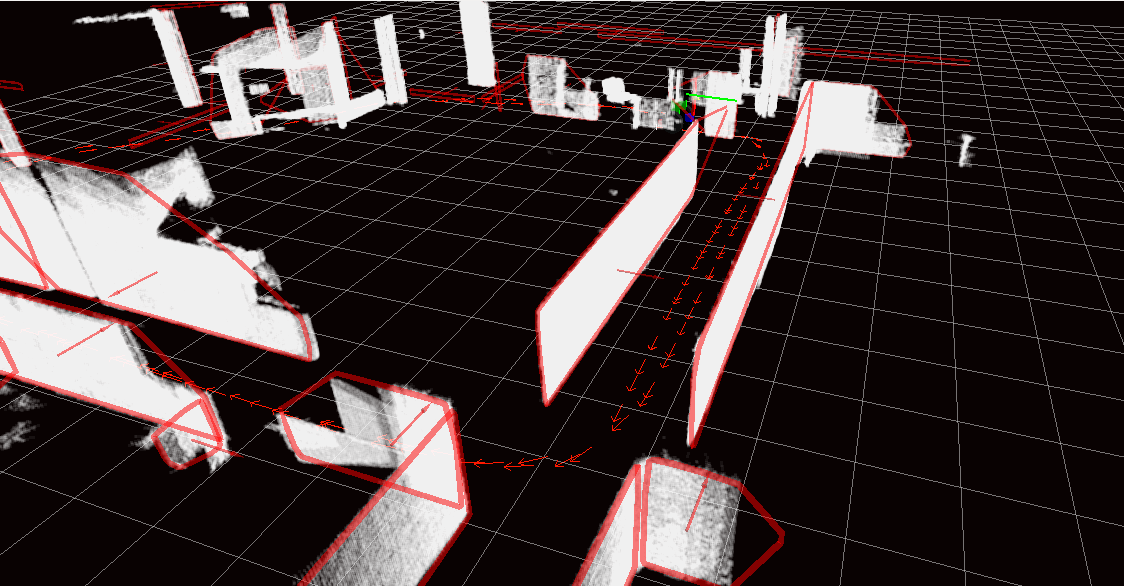
\includegraphics[width=0.7\textwidth]{pics/semantic_map}
\caption{An example of the type of map produced by our system. Planar features
are visible by the red convex hulls, and red normal vectors. The small red arrows on
the ground plane show the robot’s trajectory. The point clouds used to extract these
measurements are shown in white, and have been rendered in the map coordinate
frame by making use of the optimized poses from which they were taken.} 
\label{fig:semantic_map}
\end{center}
\end{figure}


Non-technical users will prefer human terms
for objects and locations when assigning tasks to robots instead of whatever indices or coordinates the robot uses to represent them in its memory. Semantic mapping offers an advantage for robots to understand task assignments given to them by human users. We allow humans to label planar landmarks that is automatically acquired during the SLAM process, as described in Section \ref{sec:interactive_map_labeling}. Users provide navigation goals in terms of these labeled landmarks. Our approach of finding goal points for a given planar landmark will be discussed in Section \ref{sec:finding_the_goal_point}.

Planar landmarks provide semantic information about the space, as vertical planes correspond to walls, showing how space is partitioned, while horizontal planes correspond to tables and shelves, where objects of interest may occur. We describe in Section \ref{sec:door_signs} how higher level objects, specifically door signs, can be used as landmarks in SLAM.  We further explore in Section \ref{sec:following_door_passing} how detection of door signs, therefore existence of doors, can be used for robot navigation.

\subsection{Plane Landmarks}

We believe that feature-based maps are suitable for containing task-relevant information for service robots. For example, a home service robot might need to know
about the locations of structures such as the kitchen table and countertops, cupboards and shelves. Structures such as walls could be used to better understand how space is
structured and partitioned. We describe a SLAM system capable of creating maps of
the locations and extents of planar surfaces in the environment using both 3D and 2D landmarks.

Our SLAM implementation makes use of the GTSAM library \cite{dellaert2006square}. This library
represents the graph SLAM problem with a factor graph which relates landmarks to
robot poses through factors. GTSAM builds a factor graph of nonlinear measurements. Our approach involves using multiple types of landmark measurements as factors of nonlinear measurements. Planar surfaces can be detected in point cloud data generated by 3D sensors including tilting laser range finders, or RGB-D cameras such as the Microsoft Kinect or Asus Xtion. An example of a map produced
by our system is shown in Figure \ref{fig:semantic_map}.

A plane can be represented by the well known equation:
$$ax + by + cz + d = 0$$
In this work, we make use of this representation, while additionally representing
the plane’s extent by calculating the convex hull of the observed points. While only
the plane normal and perpendicular distance are used for to correct the robot trajectory in SLAM, it is essential to keep track of the extent of planar patches, as many
coplanar surfaces can exist in indoor environments, and we would like to represent
these as distinct entities. We therefore represent planes as:
$$p = [n, hull]$$ 

where:
$$n = [a, b, c, d]$$ and \textit{hull} is a point cloud consisting of the vertices of the plane’s convex hull. As
planes are re-observed, their hulls are extended with the hull observed in the new
measurements. That is, the measured hull is projected onto the newly optimized
landmark’s plane using its normal, and a new convex hull is calculated for the sum
of the vertices in the landmark hull and the measurement’s projected hull. In this
way, the convex hull of a landmark can grow as additional portions of the plane are
observed.

We use a Joint Compatibility Branch and Bound (JCBB) technique for data association \cite{neira2001data}. JCBB works by evaluating the joint
probability over the set of interpretation trees of the measurements seen by the robot
at one pose. The output of the algorithm is the most likely interpretation tree for
the set of measurements. We are able to evaluate the probability of an interpretation
tree quickly by marginalizing out the irrelevant portions of the graph of poses and features. The branch and bound recursion structure from the EKF formulation is
used in our implementation.

Given a robot pose $X_r$, a transform from the map frame to the robot frame in the form of $(R, \vec{t})$, a previously
observed feature in the map frame $(\vec{n}, d)$ and a measured plane $(\vec{n}_m , \vec{d}_m )$, the measurement function $h$ is given by:

$$h=\bigg(
\begin{array}{c}
R^T*\vec{n}\\
\ \langle \vec{n},t\rangle + d \\
\end{array}
\bigg) -
\bigg(
\begin{array}{c}
\vec{n}_m\\
\ d_m\\
\end{array}
\bigg)
$$

The Jacobian with respect to the robot pose is then given by:

\begin{align}
\frac{\partial h}{\partial X_r}
 =
\begin{bmatrix} 
 0 & -n_a & n_b\\
 n_a & 0 & -n_c & [0]\\
 -n_b & n_c & 0\\
 0 & 0 & 0 & \vec{n}^T
\end{bmatrix}
\end{align}

The Jacobian with respect to the landmark is given by:

\begin{align}
\frac{\partial h}{\partial n_{map}}
 =
\begin{bmatrix} 
 [R_r] & \vec{0}\\
 \vec{X_r^T} & 1
\end{bmatrix}
\end{align}

Using this measurement function and its associated Jacobians, we can utilize planar normals and perpendicular distances as landmarks in our SLAM system. During
optimization, the landmark poses and robot trajectory are optimized.

\subsection{Object Landmarks: Door Signs}
\label{sec:door_signs}

The previous section introduced how we use planar landmarks for SLAM. In this section, we present a method for using a learned object classifier in a SLAM context to provide measurements suitable for mapping.

First, walls are extracted from straight lines in the laser scan. We use a
RANSAC technique to extract lines from the laser data. Only lines which are longer than a certain threshold are passed to the mapper as measurements.

\begin{figure}[ht!]
\begin{center}
\centering
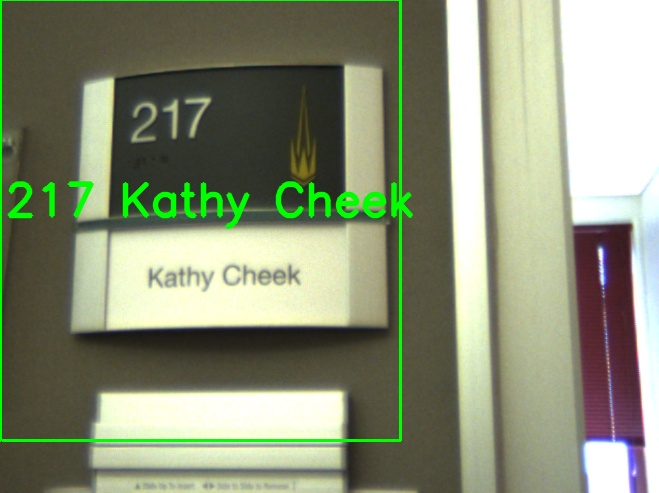
\includegraphics[width=0.3\textwidth]{pics/door_sign}
\caption{This sign is recognized and a measurement is made in the mapper. GoogleGoggles has read both the room number and the text, so this sign can be used for
data association.} 
\label{fig:door_sign}
\end{center}
\end{figure}

The door-sign-detector module makes use of a Support Vector Machine (SVM) classifier, trained on Histogram of Oriented
Gradient (HOG) features. If an image region
is classified as a sign by the SVM, then a query is made from this image region to
the GoogleGoggles server. If GoogleGoggles is able to read any text on the sign, then
it will be returned to us in a response packet. Detected signs with decoded text are
then published as measurements that can be used by the mapper. The measurements
consist of the pixel location in the image of the detected region’s centroid, the im-
age patch corresponding to the detected region, and the text string returned from
GoogleGoggles. An example detection of a door sign is shown in Figure \ref{fig:door_sign}.

Measurements generated by the door sign detector and laser line extractor modules are added as non-linear measurements to the factor graph. At the time of this study, we did not have a RGD-B sensor on the robot. Therefore, measurements were made on the 3D coordinates of the back-projected image location directly. Range is recovered by finding the laser beam from the head laser which
projects most closely to the image coordinates of the sign. This technique approximates the true range. This factor also incorporates an additional variable which corresponds
to the transformation between the robot base and the camera. 

To implement this factor in GTSAM, we must specify an error function and the
error function’s derivatives in terms of all of the variables which contribute to it. The
error function is the difference in the 3D position of the predicted location of the sign
from the measured value given by the recognition module. 

\section{Interactive Map Labeling}
\label{sec:interactive_map_labeling}

There are several methods to support the annotation of entities in a robot map. For example, while the robot is building its representation of the environment, it can recognize objects or landmarks such as doors, tables, rooms and automatically add these features to its map. Even though such a system would be useful, it may wrongly label some objects. In that case, the correct label can be provided by a human with an interactive system. Custom labels would also allow custom annotations such as ''Joe's Room".


\begin{figure}[ht!]
\begin{center}
\centering
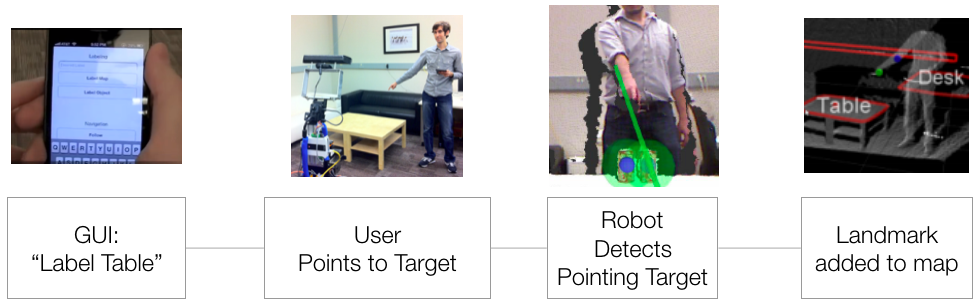
\includegraphics[width=\textwidth]{pics/labeling_flow}
\caption{Steps for interactively labeling a landmark in the semantic map. First, the user activates person following using the app. User 
stops nearby the target landmark, and enters the requested label using the app. Then the user performes a pointing gesture toward the target and waits for acknowledgement. Robot assesses the likelihood of nearby objects being the intended target, and asks for confirmation if ambiguity is detected. Finally, a string label is attached to the corresponding landmark in the semantic map.} 
\label{fig:labeling_flow}
\end{center}
\end{figure}


We presented our method for building semantic maps in Section \ref{sec:slam_and_semantic_mapping}. We will assume that we have a metric and semantic map for the rest of this paper for simplicity. To enable a common ground between the humans and the robot, we developed an interactive procedure to annotate landmarks in the semantic map. In this procedure, the person guides the robot to the landmark of interest first and refers to the landmark of interest by pointing at it. The steps for labeling a landmark is shown in Figure \ref{fig:labeling_flow}. The robot follows the user around between labeling of landmarks. This allows the user to guide the robot to virtually any location in the environment. Our interactive map labeling approach was previously described in \cite{trevor2012interactive}.

For the rest of this section, we describe the sub-components necessary to realize interactive labeling, namely person following (Section \ref{sec:person_following}), pointing gestures (Section \ref{sec:pointing_gestures}) and object labeling (Section \ref{sec:object_labeling}).

\subsection{Person Following}
\label{sec:person_following}

The robot has to continously estimate the position of the user in real-time for robust person following. We focus on tracking people who are either walking or standing, as these are the two most common human poses around a mobile robot. The reason for using multiple detectors for the person tracking system is to increase the robustness and provide $360^{\circ}$ coverage around the robot. Below are the brief descriptions of the person detection methods:

1) Leg Detector: A front-facing laser scanner at ankle height (Hokuyo UTM 30-LX) is used. We trained a leg classifier using three geometric features: Width, Circularity and Inscribed Angle Variance \cite{xavier2005fast}. We find a distance score for each candidate segment using the weighted sum of the distance to each feature and then threshold the score for detection.

2) Torso Detector: A back-facing Hokuyo laser scanner, placed at torso-level
is used for this detector. We model
the human torso as an ellipse and fit each segment in the laser an ellipse. The ellipse fitting approach always returns a result, even for bad data. In addition to the geometric features we use for legs, we use two additional features for torso detection: The horizontal and vertical axes of the fitted ellipse. Similar to leg detection, we use a threshold test for the detection result.

The output of the detectors are input to a state estimation module. Using a state predictor for human movement has two advantages. First, the predicted trajectories are smoother than
raw detections. Smooth tracking helps the robot maintain consistent trajectories
for person following. Second, it provides a posterior estimate that can be used for data association when there is a lack of
matching detections. This allows the tracker to handle temporary occlusions. We use
a Linear Kalman Filter (KF) with constant velocity model to estimate the position and velocity of a person. We used a KF for tracking because it has acceptable tracking performance and is computationally cheap, which is important in real-time applications.

For person following, the robot uses the most probable location of the KF, which is the mean of the Gaussian distribution. We use Dynamic Window Approach (DWA) \cite{fox1997dynamic} at the core of our planner to sample velocity and acceleration-bounded trajectories, with the modification of using time as an additional dimension. DWA forward-simulates allowable velocities and chooses an action that optimizes a function that will create a goal-directed behavior while avoiding obstacles. Our approach projects the future locations of the target, creates a tree of trajectories, and scores each tree node according to a goal function, which is a function of the relative pose of the robot with respect to the human. Our planner takes the laser scan measurement, predicted positions of the person, and the number of time steps to plan as input and outputs a sequence of actions. A robot configuration at time $t$ is expressed as \(q^t=(x^t,y^t,\theta^t,v^t,\omega^t)^\mathrm{T}\), where $x^t$ and $y^t$ denote positions, $\theta^t$ is the orientation, $v^t$ and $w^t$ are the linear and angular velocities at time $t$. The person configuration \(p^t\) is defined the same way. An action of the robot is defined as a velocity command for some duration: $a(t,\Delta t)=(v^t_a,\omega^t_a,\Delta t)$. We assume a unicycle kinematics model for trajectory sampling. Using this model, we generate a tree up to a fixed depth, starting from the current configuration of the robot. A tree node consists of a robot configuration as well as the information about the previous action and parent node. Every depth of the tree corresponds to a discretized time slice. Therefore, every action taken in the planning phase advances the time by a fixed amount. This enables the planner to consider future steps of the person and simulate what is likely to happen in the future. The planner uses depth-limited Breadth First Search (BFS) to search all the trajectories in the generated tree and determines the trajectory that will give the robot the maximum utility over a fixed time in the future. Given the robot and person configuration at some particular time, goal function \(0 \leq g(q^t,p^t) \leq 1\) determines how desirable the situation is for the task. Goal function can be defined in any way and provides flexibility to the navigation behavior designer. We assume that it is desirable for the robot to follow from behind as it would give the robot a better chance to predict the human's motions and implicitly mimic human's path, which is known to be obstacle free. We report our results on this person following method in Section \ref{sec:eval_person_following}. In previous work, we applied this following method on an autonomous telepresence robot \cite{cosgun2013autonomous}. 

Another important capability to enable interactive labeling is to be able to refer to the same landmarks in the environment. Our design involves the person extending his/her arm and point at the landmark of interest. The method for detecting the pointing target is described next.


\subsection{Pointing Gestures}
\label{sec:pointing_gestures}

In this section, we present an uncertainty model for estimating pointing gesture targets, based on previous work \cite{cosgun2015did}. Estimating this uncertainty allows us to interpret whether a pointing gesture is ambiguous or not, when objects are too close to one another. We model the uncertainty of pointing gestures using a spherical coordinate system. We use this model to determine the correct pointing target, and detect when there is ambiguity. Two pointing methods, elbow-hand and head-hand rays, are evaluated using a 3rd party skeleton tracking algorithm, OpenNI NITE in Section \ref{sec:eval_pointing_gestures}.

We use a simple gesture detection algorithm as our focus is to estimate the gesture target given that a pointing gesture was performed. Using the skeleton data, pointing gestures are recognized if a human's forearm makes more than a fixed angle with the vertical axis and elbow and hand joints stay almost stationary for a fixed duration. Gesture detection is activated only after the user requests a labeling action. This design is intended to reduce false positive detections.

We represent a pointing ray in two angles: a ``horizontal" sense we denote as $\theta$ and a ``vertical" sense we denote as $\psi$. We first attach a coordinate frame to the hand point, with its z-axis oriented in either Elbow-hand $\vec{v}_{eh}$ or Head-Hand $\vec{v}_{hh}$ directions. The hand was chosen as the origin for this coordinate system because both of head-hand and elbow-hand pointing methods include the user's hand. The transformation between the sensor frame and the hand frame $^{sensor}T_{hand}$ is calculated by using an angle-axis rotation method. An illustration of the hand coordinate frame for Elbow-Hand method and corresponding angles are shown graphically in Figure~\ref{fig:angle_errors}.

\begin{figure}[h!]
\centering
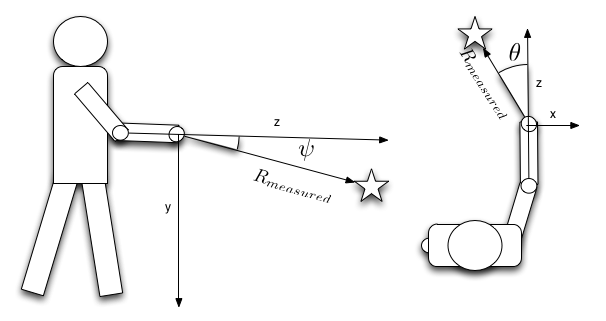
\includegraphics[width=85mm]{pics/person_angles_combined_2.png}
\caption{Vertical $(\psi)$ and horizontal $(\theta)$ angles in spherical coordinates are illustrated. A potential intended target is shown as a star. The z-axis of the hand coordinate frame is defined by either the Elbow-Hand (this example) or Head-Hand ray.}
\label{fig:angle_errors}
\end{figure}

Given this coordinate frame and a potential target point P, we first transform it to the hand frame by:
$$^{hand}p_{target} = T_{hand} * p_{target}$$
We calculate the horizontal and vertical angles for a target point as $^{hand}p_{target} = (x_{targ}, y_{targ}, z_{targ})$ follows:
$$[\theta_{target}\;\psi_{target}]=[atan2(x_{targ}, z_{targ})\;atan2(y_{targ}, z_{targ})]$$

Where $atan2(y,x)$ is a function returns the value of the angle $\arctan(\frac{y}{x})$ with the correct sign.

We estimate the likelihood of objects being the target using statistical data from previous pointing gesture observations. We observed that head-hand and elbow-hand methods returned different angle errors depending on the target location. Our approach relies on finding error statistics of these approaches, and compensating the error when the target object is searched for. First, given a set of prior pointing observations, we calculate the mean and variance of the vertical and horizontal angle errors for each pointing method. This analysis will be presented in Section \ref{sec:eval_pointing_gestures}. Given an input gesture, we apply correction to the pointing direction and find the Mahalanobis distance to each object in the scene.

When a pointing gesture is recognized, and the angle pair $[\theta_{target}\;\psi_{target}]$ is found, and then a correction is applied by subtracting the mean terms from measured angles:
$$[\theta_{cor}\;\;\psi_{cor}]=[\theta_{target}-\mu_{\theta}\;\;\;\psi_{target}-\mu_{\psi}]$$
 
We also compute a covariance matrix for angle errors in this spherical coordinate system: 
$$S_{type} = \begin{bmatrix}
\sigma_{\theta}&0\\ 0&\sigma_{\psi}
\end{bmatrix} $$

We get the values for $\mu_{\theta}, \mu_{\psi}, \sigma_{\theta} ,\sigma_{\psi}$ from Table~\ref{table:pointing_error_stats} for the corresponding gesture type and closest target location. We then compute the mahalanobis distance to the target by:
$$D_{mah}(target,method)=\sqrt{ [\theta_{cor}\;\psi_{cor}]^T S_{method}^{-1} [\theta_{cor}\;\psi_{cor}]}$$
 
We use $D_{mah}$ to estimate which target or object is intended. We consider two use cases: the objects are represented as a point or a point cloud. For point targets, we first filter out targets that have a Mahalanobis distance larger than a threshold $D_{mah} > D_{thresh}$. If none of the targets has a $D_{mah}$ lower than the threshold, then we decide the user did not point to any targets. If there are multiple targets that has $D_{mah} \leq D_{thresh}$ , then we determine ambiguity by employing a ratio test. The ratio of the least $D_{mah}$ and the second-least $D_{mah}$ among all targets is compared with a threshold to determine if there is ambiguity. If the ratio is higher than a threshold, then the robot can resort to additional action, such as initiating a dialogue to ask or confirm the intended object.


\subsection{Labeling Object Models}
\label{sec:object_labeling}

Our method supports labeling two types of landmarks: planar surfaces and objects. The UI shows two labeling buttons ''Label Object" and ''Label Planar Surface", so that the robot knows what the user is intending to label. Section \ref{sec:pointing_gestures} demonstrated how point targets or point cloud targets can be referenced via pointing gestures. The referenced object is then annotated
with the label entered by the user, and can then be recognized later as described in our previous work \cite{trevor2013interactive}. Figure \ref{fig:labeling_objects} shows the steps the robot executes for this task. Service robotic tasks that use such a map can then reference the object
by label, rather than generating a more complex referring expression (e.g. “the large
object” or “the object on the left”).

\begin{figure}
\begin{center}
\begin{minipage}{160mm}
\subfigure[]{
\resizebox*{5.5cm}{!}{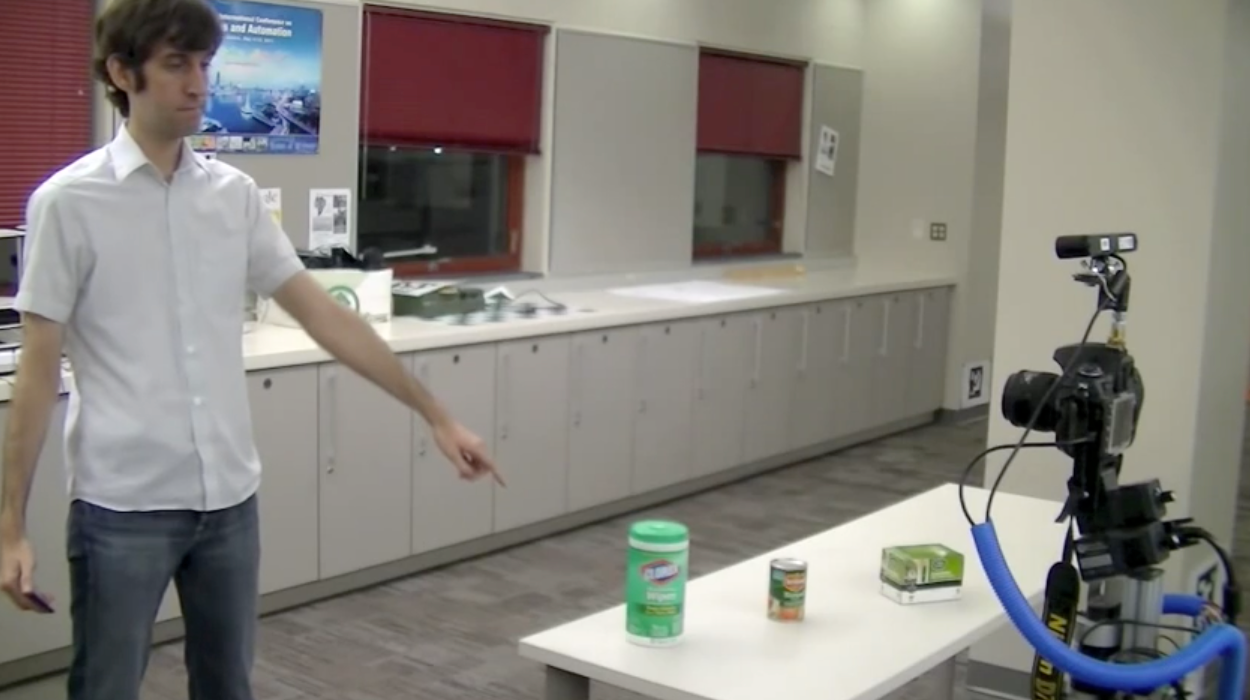
\includegraphics{pics/obj_label_0}}}
\subfigure[]{
\resizebox*{5.8cm}{!}{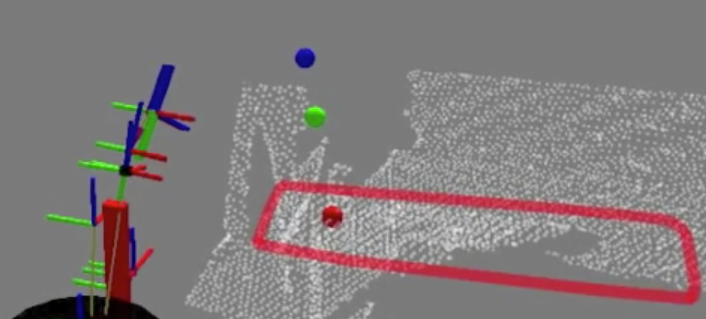
\includegraphics{pics/obj_label_1}}}
\subfigure[]{
\resizebox*{4cm}{!}{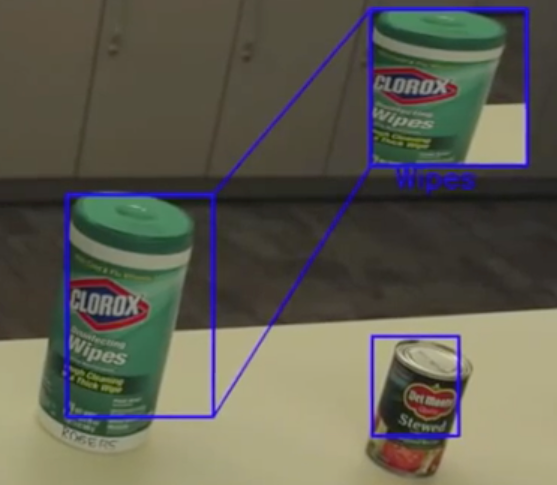
\includegraphics{pics/obj_label_2}}}
\caption{a) A user pointing at an object. b) A detected pointing gesture
(blue and green spheres), and referenced object (red sphere). c) Features are
extracted from an image patch corresponding to the cluster, and annotated with the
provided label.} \label{fig:labeling_objects}
\end{minipage}
\end{center}
\end{figure}


\section{Evaluation of Sub-Components}
\label{sec:evaluation}

In this section, we evaluate two of the core sub-components that enables building interactive semantic maps. In Section \ref{sec:eval_person_following} we analyze the person following behavior and in Section \ref{sec:eval_pointing_gestures} we evaluate our pointing gesture target estimation method.

\subsection{Evaluation of Person Following}
\label{sec:eval_person_following}

In this section, we report on an analysis of the person following sub-component. In our experiments, the robot followed 7 people for 3 laps and we logged the total distance robot followed the person and the average distance to the person. Users did not have prior experience with the robot and was asked to walk in a corridor while the robot is following them. A lap consisted of leaving the starting point, going to an intermediate point at the end of the corridor and coming back to the starting point from the same path. Table \ref{tab:perf} shows the data pertaining this study. In total, the robot followed people for about 1.2km. The average distance between the person and the robot across all 7 runs was 1.16m (Table \ref{tab:perf}).

\begin{table}[!h]
\begin{center}
  \begin{tabular}{| r || r | r |}
    \hline
    Subject \# & Distance (m) & Avg. Dist to Person (m) \\ \hline 
    1 & 171.4  & 1.1\\ \hline
    2 & 161.8  & 1.13\\ \hline
    3 & 160.4  & 1.14\\ \hline
    4 & 169.9  & 1.25\\ \hline
    5 & 174.2  & 1.04\\ \hline
    6 & 166.2  & 1.3\\ \hline
    7 & 171.5  & 1.2\\ \hline
  \end{tabular}
\label{tab:perf}
\end{center}
\caption {Performance of the person follower on 7 subjects}
\end{table}


\begin{figure}[ht!]
\centering
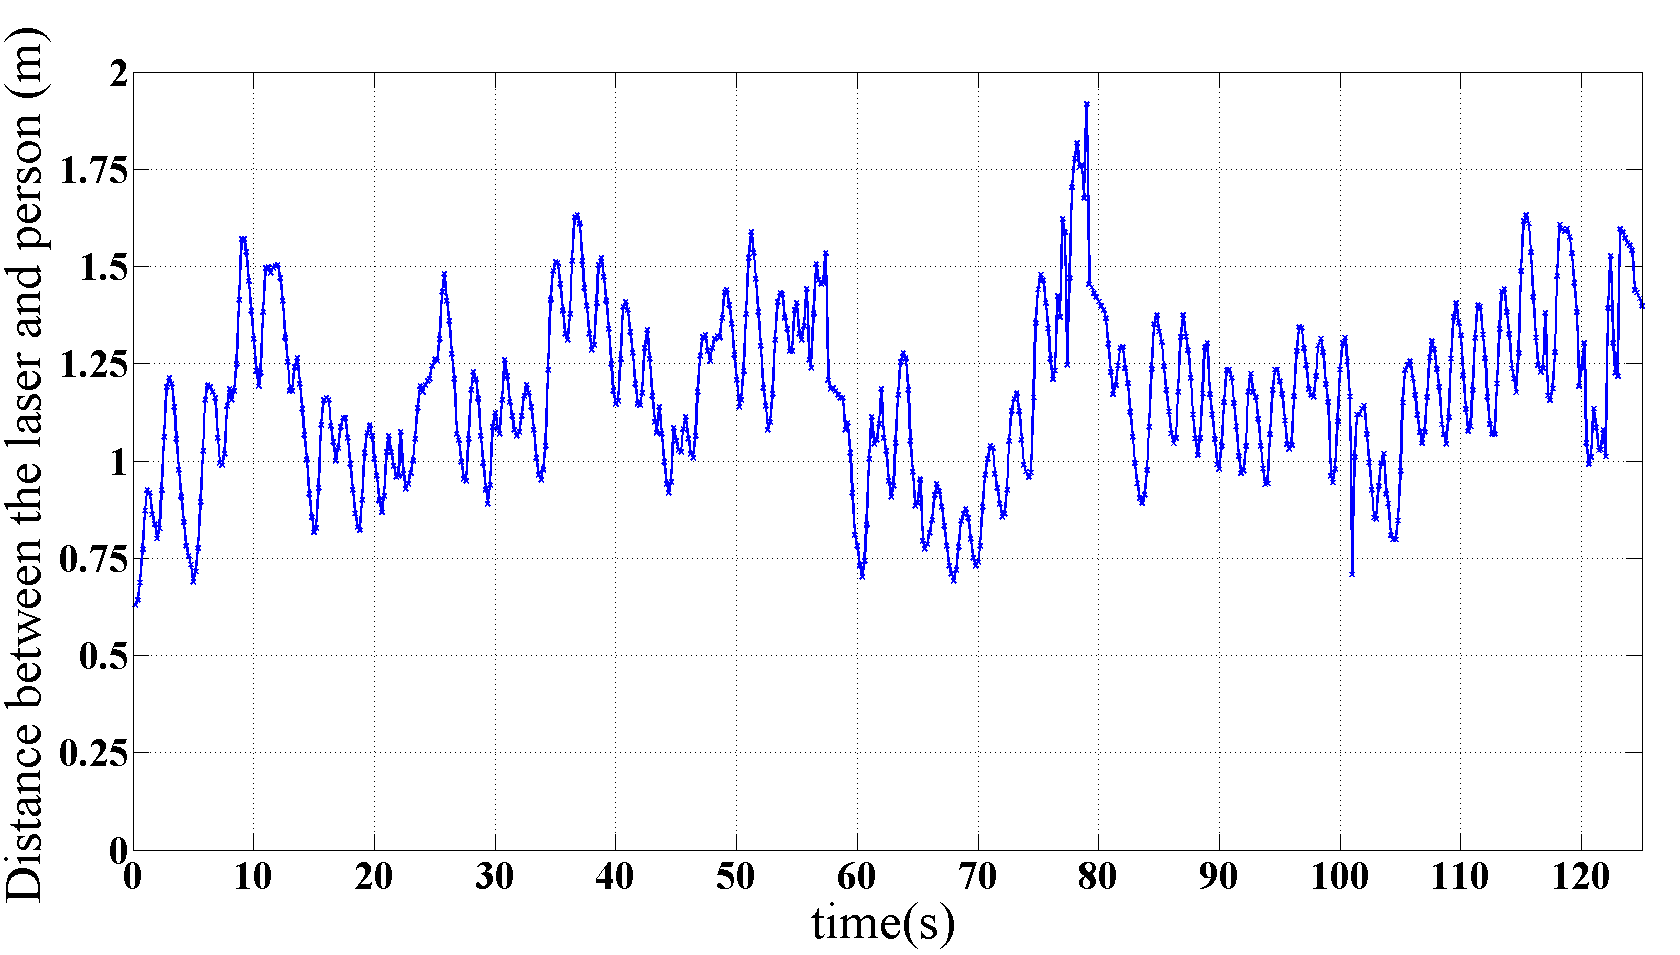
\includegraphics[width=0.65\textwidth]{pics/following_result}
\caption{Following distance as a function of time for one of the person following experiments.}
\label{fig:graph}
\end{figure}

Figure \ref{fig:graph} plots the time versus following distance for a sample run that consists of 1 lap. At $t=0$, the following is initiated and robot leaves the starting point. Around $t=8s$, the robot and the person start making a right turn. The sudden drop in following distance at $t=57.2$ signifies that the robot lost track of the person and the person tracker is reinitialized. At $t=65.6s$, the intermediate point at the end of the corridor is reached so the person makes a 180$^\circ$ turn. The robot is close to the person (about $0.75m$) around this time because the robot is rotating around itself while the person is turning back. Between $t=70$ and $t=80s$, the person walks faster than the robot, so the following distance reaches to a maximum of $1.91m$. At $t=79.8s$, the person is lost again. Around $t=115s$, the robot and the person make a left turn. The lap ends at $t=124s$. Note that the high frequency fluctuation of the following distance is a result of tracking only a single leg.


\subsection{Evaluation of Pointing Gestures}
\label{sec:eval_pointing_gestures}

To evaluate the accuracy of pointing gesture target detection, we first find the error statistics for pointing gestures, then apply it to a scenario for distinguishing two objects with varying separation.

\begin{figure}[thpb]
\centering
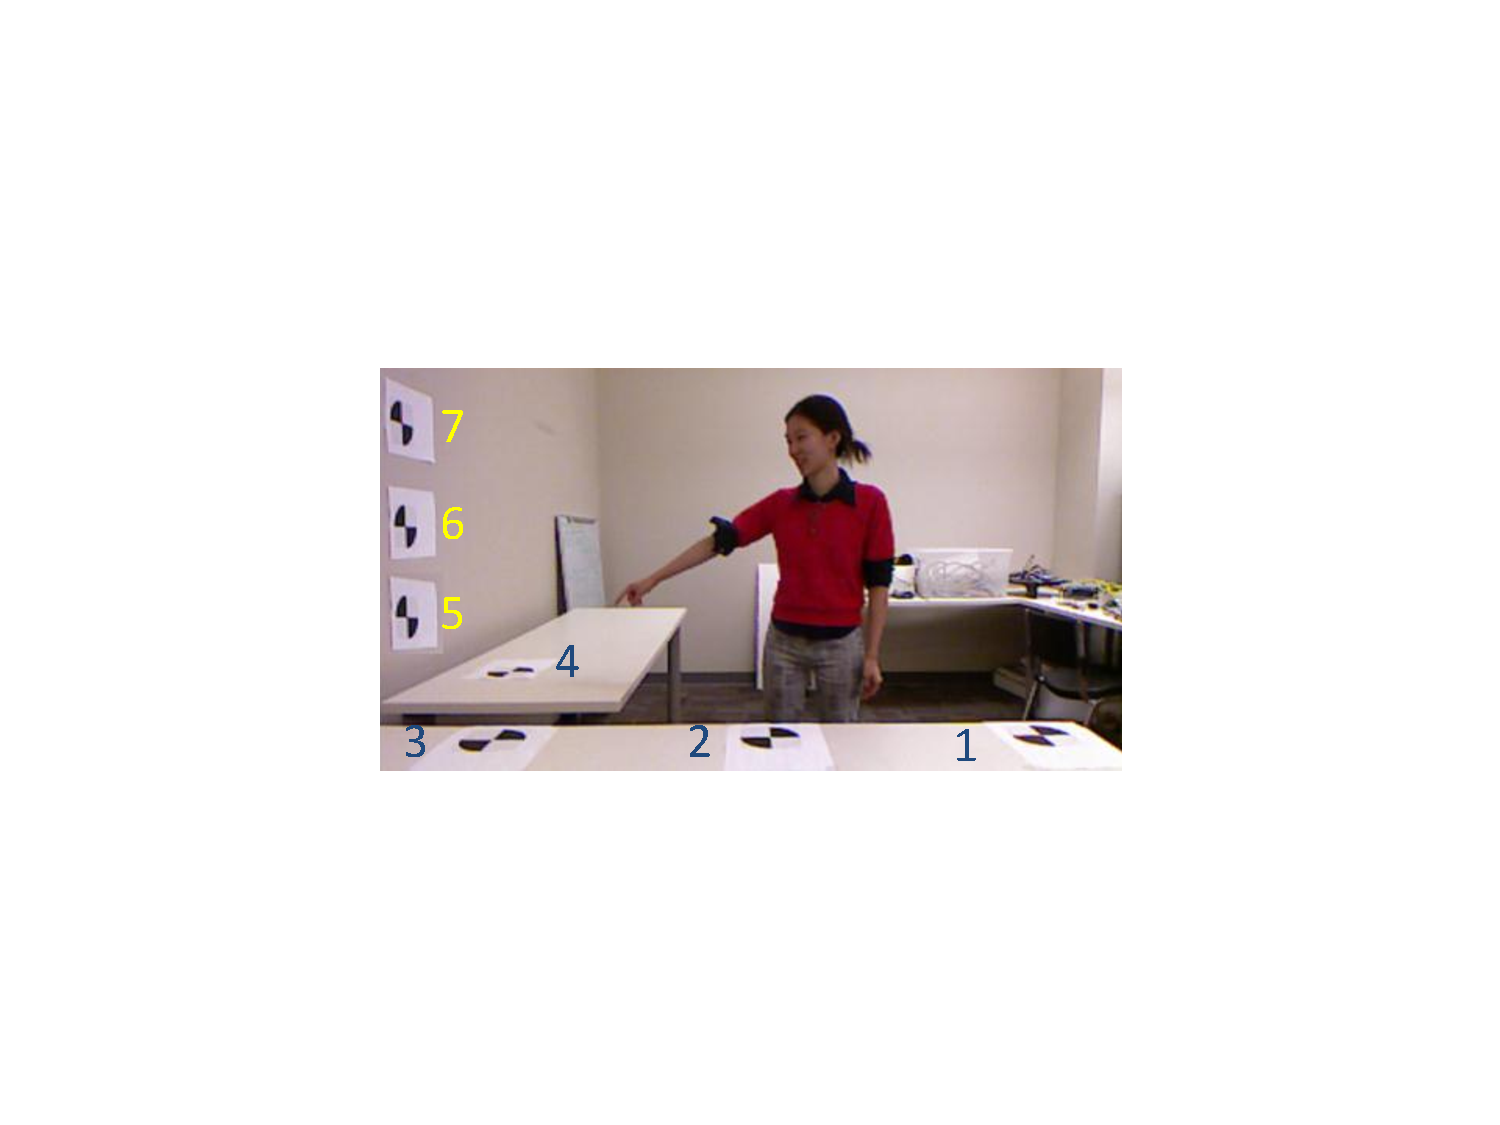
\includegraphics[width=65mm]{pics/data_collection_crop}
\caption{Our study involved 6 users that pointed to 7 targets while being recorded using 30 frames per target.}
\label{fig:ground_truth_targets}
\end{figure}

We collected data from 6 users, with 7 targets, where people pointed at each target with their right arms (Figure \ref{fig:ground_truth_targets}). Our use case is on a mobile robot platform capable of positioning itself relative to the user.  For this reason, we can assume that the user is always centered in the image, as the robot can easily rotate to face the user and can position itself at a desired distance from the user. The ground truth points, represented in the camera frame is found by first finding the pixel values of targets using a corner detector, extending a virtual ray from camera origin to a target and finding the intersection point to the supporting plane, which is extracted from the point cloud data. We computed the mean and standard deviations of the angular errors in the spherical coordinate system for each pointing gesture method and target. 



\begin{table}[ht!]
\centering
\begin{tabular}{c| @{} x{0.9cm}| @{} x{0.9cm}| @{} x{0.9cm}| @{} x{0.9cm}| @{} x{0.9cm}| @{} x{0.9cm}| @{} x{0.9cm}| @{} p{0.9cm}|}
\cline{2-9}
& \multicolumn{4}{c|}{Target 2} & \multicolumn{4}{c|}{All Targets} \\ \cline{2-9}
& \multicolumn{2}{c|}{$\theta$} & \multicolumn{2}{c|}{$\psi$} & \multicolumn{2}{c|}{$\theta$} & \multicolumn{2}{c|}{$\psi$} \\ \cline{2-9}
& \footnotesize{$\mu$} & \footnotesize{$\sigma$} & \footnotesize{$\mu$} & \footnotesize{$\sigma$} & \footnotesize{$\mu$} & \footnotesize{$\sigma$} & \footnotesize{$\mu$} & \footnotesize{$\sigma$} \\ \hline

\multicolumn{1}{ |c|}{\textbf{\scriptsize{Elbow-Hand}}}& -3.8 & 6.6  & 11.3 & 10.9  & -11.2 & 7.6  & 9.6 &\multicolumn{1}{r|}{6.3} \\ \hline
\multicolumn{1}{ |c|}{\textbf{\scriptsize{Head-Hand}}}& 10.2  & 6.7  & -5.7 & 8.0   & -2.4 & 9.6  & -5.3 &\multicolumn{1}{r|}{6.4} \\ \hline
\end{tabular}
\caption{$\mu$ and $\sigma$ of angular errors (in degrees) are given for Target 2 and across all targets. Error statistics of Table 2 was used for the object separation evaluation. Reader is referred to \cite{cosgun2015did} for the complete table.}
\label{table:pointing_error_stats}
\end{table}


The error statistics for Target 2 and across all targets are given in Table \ref{table:pointing_error_stats}. The reason for reporting Target 2 only is that we use the error statistics of that target for the object separation study. From the data, we can tell that for the elbow-hand pointing method users typically point about $11^\circ$ to the left of the intended target direction, and about $9^\circ$ above the target direction. Similarly, the data from the head-hand pointing method reports that users typically point about $2^\circ$ to the left of the intended pointing direction, but with a higher standard deviation than the elbow-hand method.  On average, the vertical angle $\psi$ was about $5^\circ$ below the intended direction with a higher standard deviation than the elbow-hand method. The horizontal angle $\theta$ has a higher variation than the vertical angle $\psi$.  Examining the errors for individual target locations shows that this error changes significantly with the target location. Therefore for a given target location, we first choose the closest target category in our data set, and use the corresponding mean and standard deviation values.


\begin{figure}[ht!]
\centering
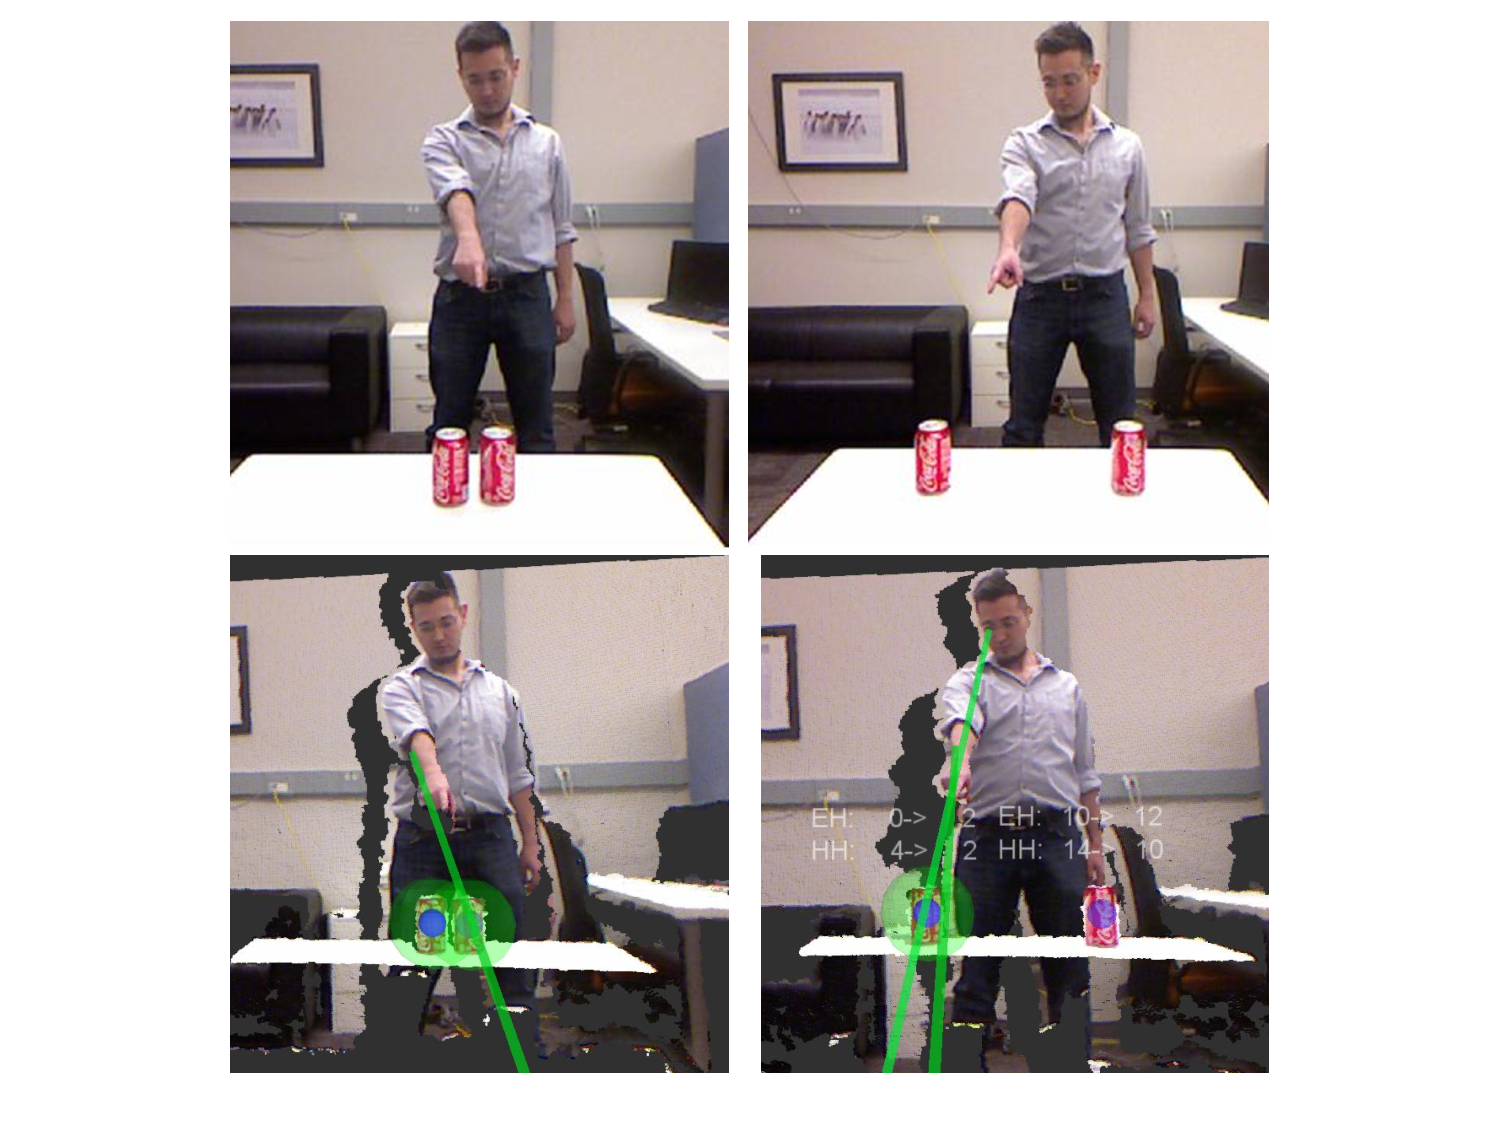
\includegraphics[width=75mm]{pics/separation_2_cropped}
\caption{Example scenarios from the object separation test is shown. Our experiments covered separations between $2cm$ (left images) and $30cm$ (right images). The object is comfortably distinguished for the $30cm$ case, whereas the intended target is ambiguous when the targets are $2cm$ apart. Second row shows the point cloud from the RGB-D camera's view. Green lines show the Elbow-Hand and Head-Hand directions whereas green circles show the objects that are within the threshold $D_{mah}<2$.}
\label{fig:separation}
\end{figure}


Next, we conducted an experiment to determine how our approach distinguished two potentially ambiguous pointing target objects. The setup consisted of a table between the robot and the person and two coke cans on the table (Figure~\ref{fig:separation}) where the separation between objects was varied. The center positions of objects were calculated in real-time by a point cloud segmentation with supporting plane assumption. The separation between objects were varied with 1 cm increments from $2 cm$ to $15 cm$ and with $5 cm$ increments between $15 cm-30 cm$. We could not conduct the experiment below $2 cm$ separation because of the limitations of our perception system. The experiment was conducted with one user, who was not in the training dataset. For each separation, the user performed five pointing gestures to each object. The person pointed to one of the objects and the Mahalanobis distance $D_{mah}$ to the intended object and the other object is calculated. Error statistics of Target 2 (Figure \ref{fig:ground_truth_targets}) was used for this experiment.


\begin{figure}[ht!]
\centering
%
        \subfigure[]{%
            \label{fig:eh_graph}
            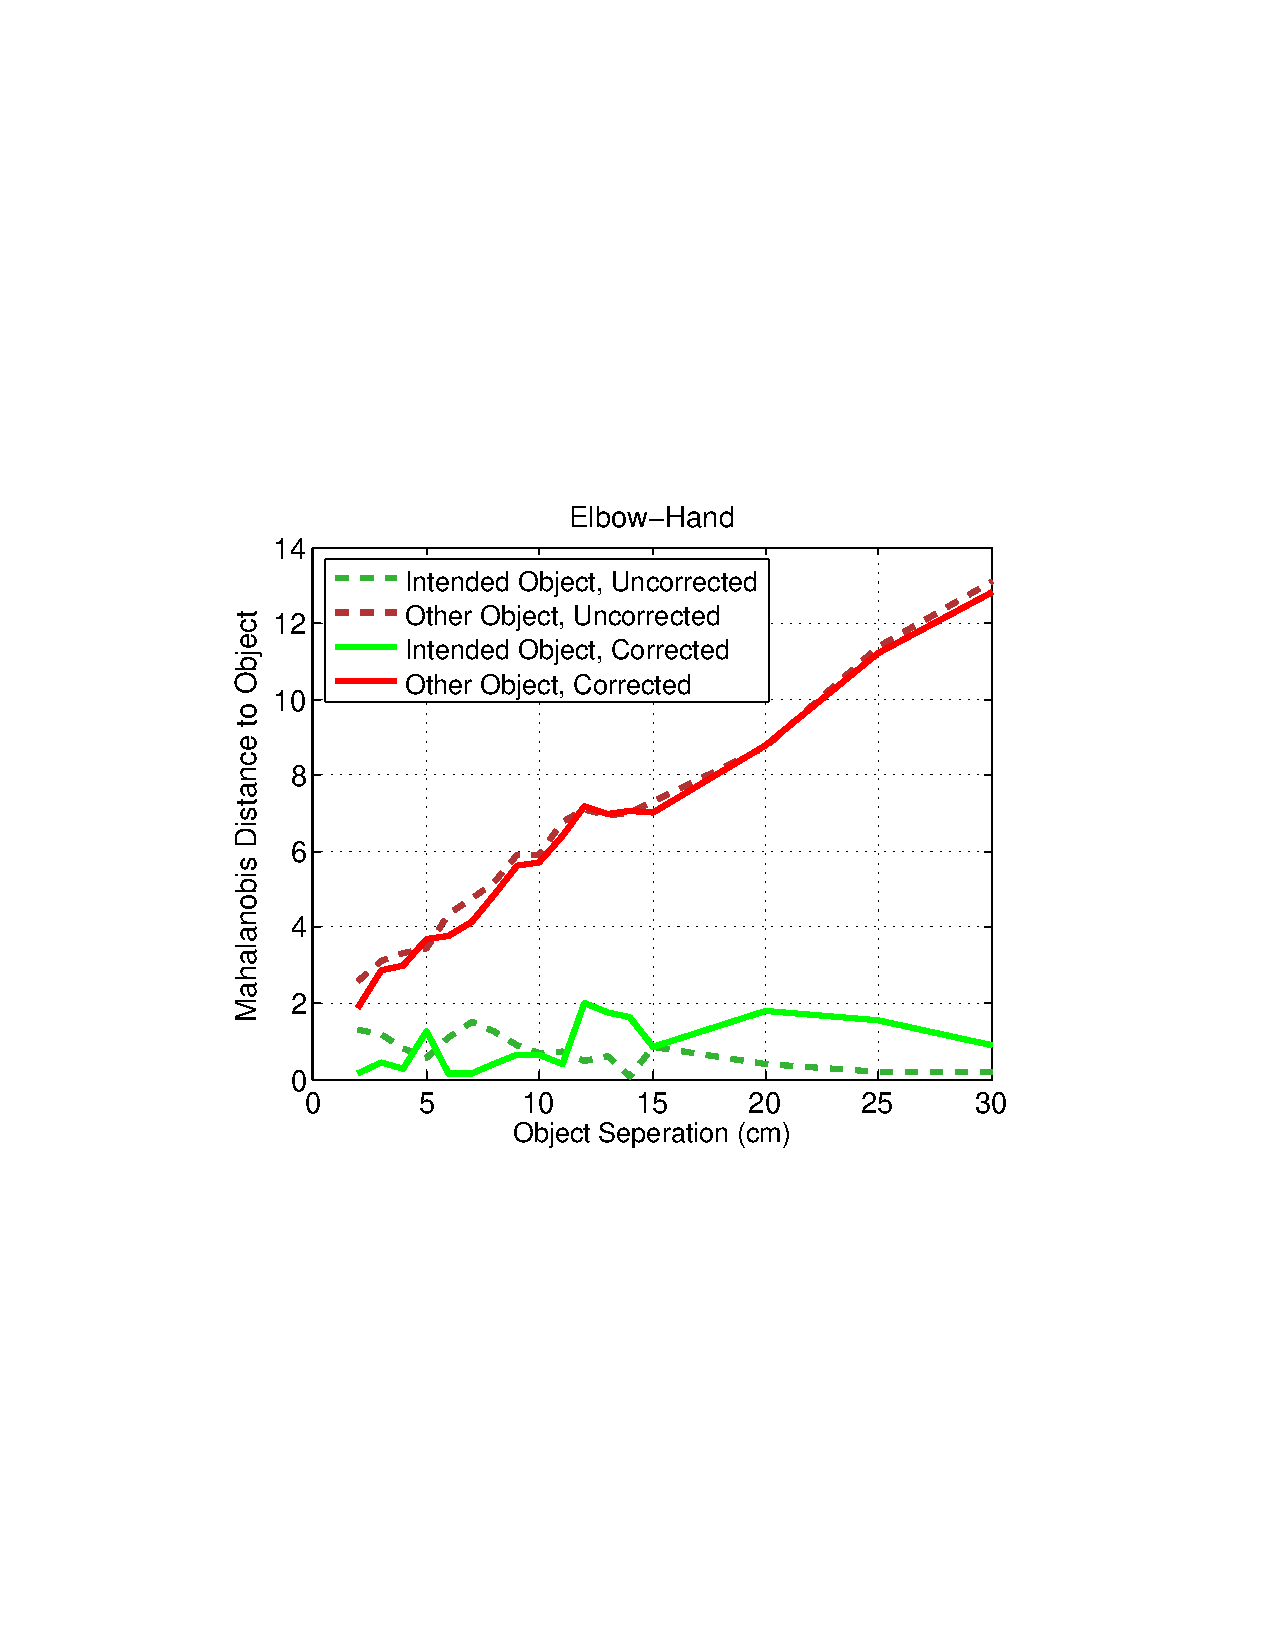
\includegraphics[width=73mm]{pics/eh_graph_crop}
        }%
        \subfigure[]{%
           \label{fig:hh_graph}
           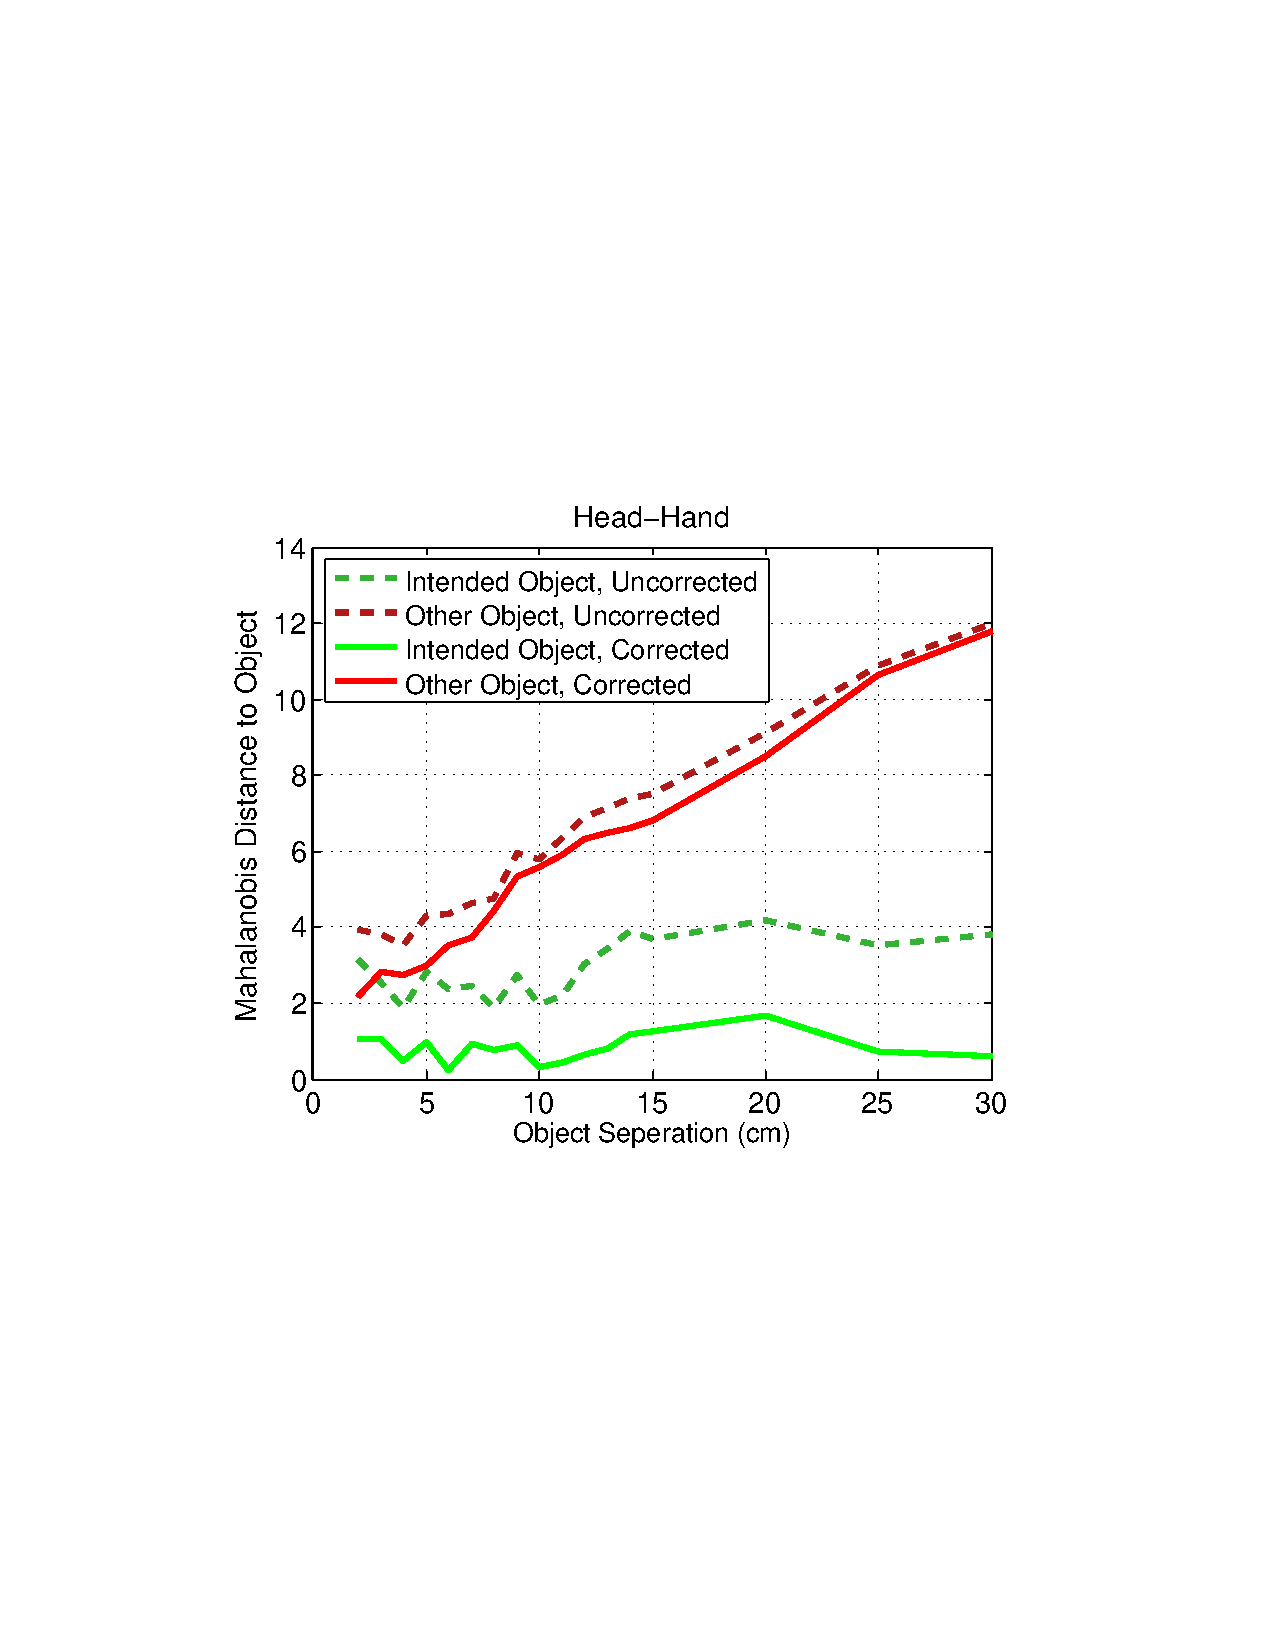
\includegraphics[width=73mm]{pics/hh_graph_crop}
        }        
    \caption{%
	Resulting Mahalanabis distances of pointing targets from the Object Separation Test is shown for a) Elbow-Hand and b) Head-Hand pointing methods. Intended object are shown in green and other object is in red. Solid lines show distances after correction is applied. Less Mahalanobis distance for intended object is better for reducing ambiguity.
     }%
   \label{fig:pointing_separation_results}
\end{figure}

The results of the object separation experiment is given for Elbow-Hand (Figure~\ref{fig:eh_graph}) and Head-Hand (Figure~\ref{fig:hh_graph}) methods. The graphs plot object separation versus the Mahalanobis distance for the intended unintended objects, for corrected and uncorrected pointing gestures. First, the Mahalanobis distance $D_{mah}$ for the intended object was always lower than the other object. The corrected $D_{mah}$ for both Elbow-Hand and Head-Hand methods for the intended object was always below 2, therefore selecting the threshold $D_{thres}=2$ is a reasonable choice. We notice that some distances for the unintended object at 2cm separation is also below $D_{mah}<2$. Therefore, when the objects are 2 cm apart, then the pointing target becomes ambiguous for this setup. For separations of 3cm or more, $D_{mah}$ of the unintended object is always over the threshold, therefore there is no ambiguity. Second, correction significantly improved Head-Hand accuracy at all separations, slightly improved Elbow-Hand between 2-12cm but slightly worsened Elbow-Hand after 12cm. Third, the Mahalanobis distance stayed generally constant for the intended object, which was expected. It linearly increased with separation distance for the other object. Fourth, patterns for both methods are fairly similar to each other, other than Head-Hand uncorrected distances being higher than Elbow-Hand.


\section{Robot Navigation using Semantic Maps}
\label{sec:robot_navigation}


Autonomous navigation is one of the most fundamental capabilities for a mobile robot. There are many approaches that achieve point-to-point autonomous navigation thanks to the advances in mapping, localization and motion planning research. Many of these algorithms are optimized to find the least-cost path, or the shortest path. However, often there are additional social factors to consider for navigation among humans. 

First, it is not natural for humans to provide the goals in exact coordinates. Instead, the robot should be able to understand goals that are expressed natural language and grounded with shared references. In our approach, users provide annotated landmarks as goals to the robot using a mobile app. Our method of goal calculation from a user query is discussed in Section \ref{sec:finding_the_goal_point}.

Second, robots should pay special attention to their motions when there are humans in the environment, or when there is a probability of encountering a human. For example, while it is acceptable for a robot to get very close to a wall, doing so to a human is socially unacceptable and unsafe. Similarly, sudden appearance of a robot can surprise humans and cause discomfort. There are many other social scenarios where the shortest path may not be optimal. Therefore context-aware path planning algorithms should treat humans and obstacles differently to enable intelligent robot behaviors. Our human-aware path planning method is described in Section \ref{sec:human_aware_path_planning}.

Third, semantic maps could be exploited to enhance navigation behaviors. Robot navigation behaviors could be tailored to the task at hand. For example, when the robot is following a person during the map labeling task, the robot choose its sub-goals to facilitate interaction. Similarly, semantic maps could be useful to negotiate passing in bottlenecks, such as door passages. We present our context-aware person following approach in Section \ref{sec:context_aware_person_following}, built on top of the person following method presented in Section \ref{sec:person_following}.

\subsection{Navigating to Labeled Landmarks}
\label{sec:navigating_to_labeled_landmarks}

\subsubsection{Finding the Goal Point}
\label{sec:finding_the_goal_point}

In our current application, the goals are either labeled landmarks or objects using a phone/tablet app. When a user enters a landmark as a navigation goal, the robot first finds a goal point in the metric map, then plans and executes a socially acceptable path toward this goal.

When a planar landmark is entered as the goal, the metric goal is chosen towards the closest edge of the plane. We first select the closest vertex on the landmark's convex hull to the robot's current position, and project it to the floor plane. We find the line between the closest vertex on the convex hull and the robot's current pose. The goal position is selected to be on this line, a meter away from the vertex. With this design, robot would reach to close proximity of the desired planar surface and be oriented towards it. This method is suitable for horizontal planes such as tables, and vertical planes alike, such as doors. An example for finding a goal pose for a uniquely labeled planar landmark is shown in Figure \ref{fig:single_plane}.

\begin{figure}[ht!]
\centering
%
        \subfigure[]{%
            \label{fig:single_plane}
            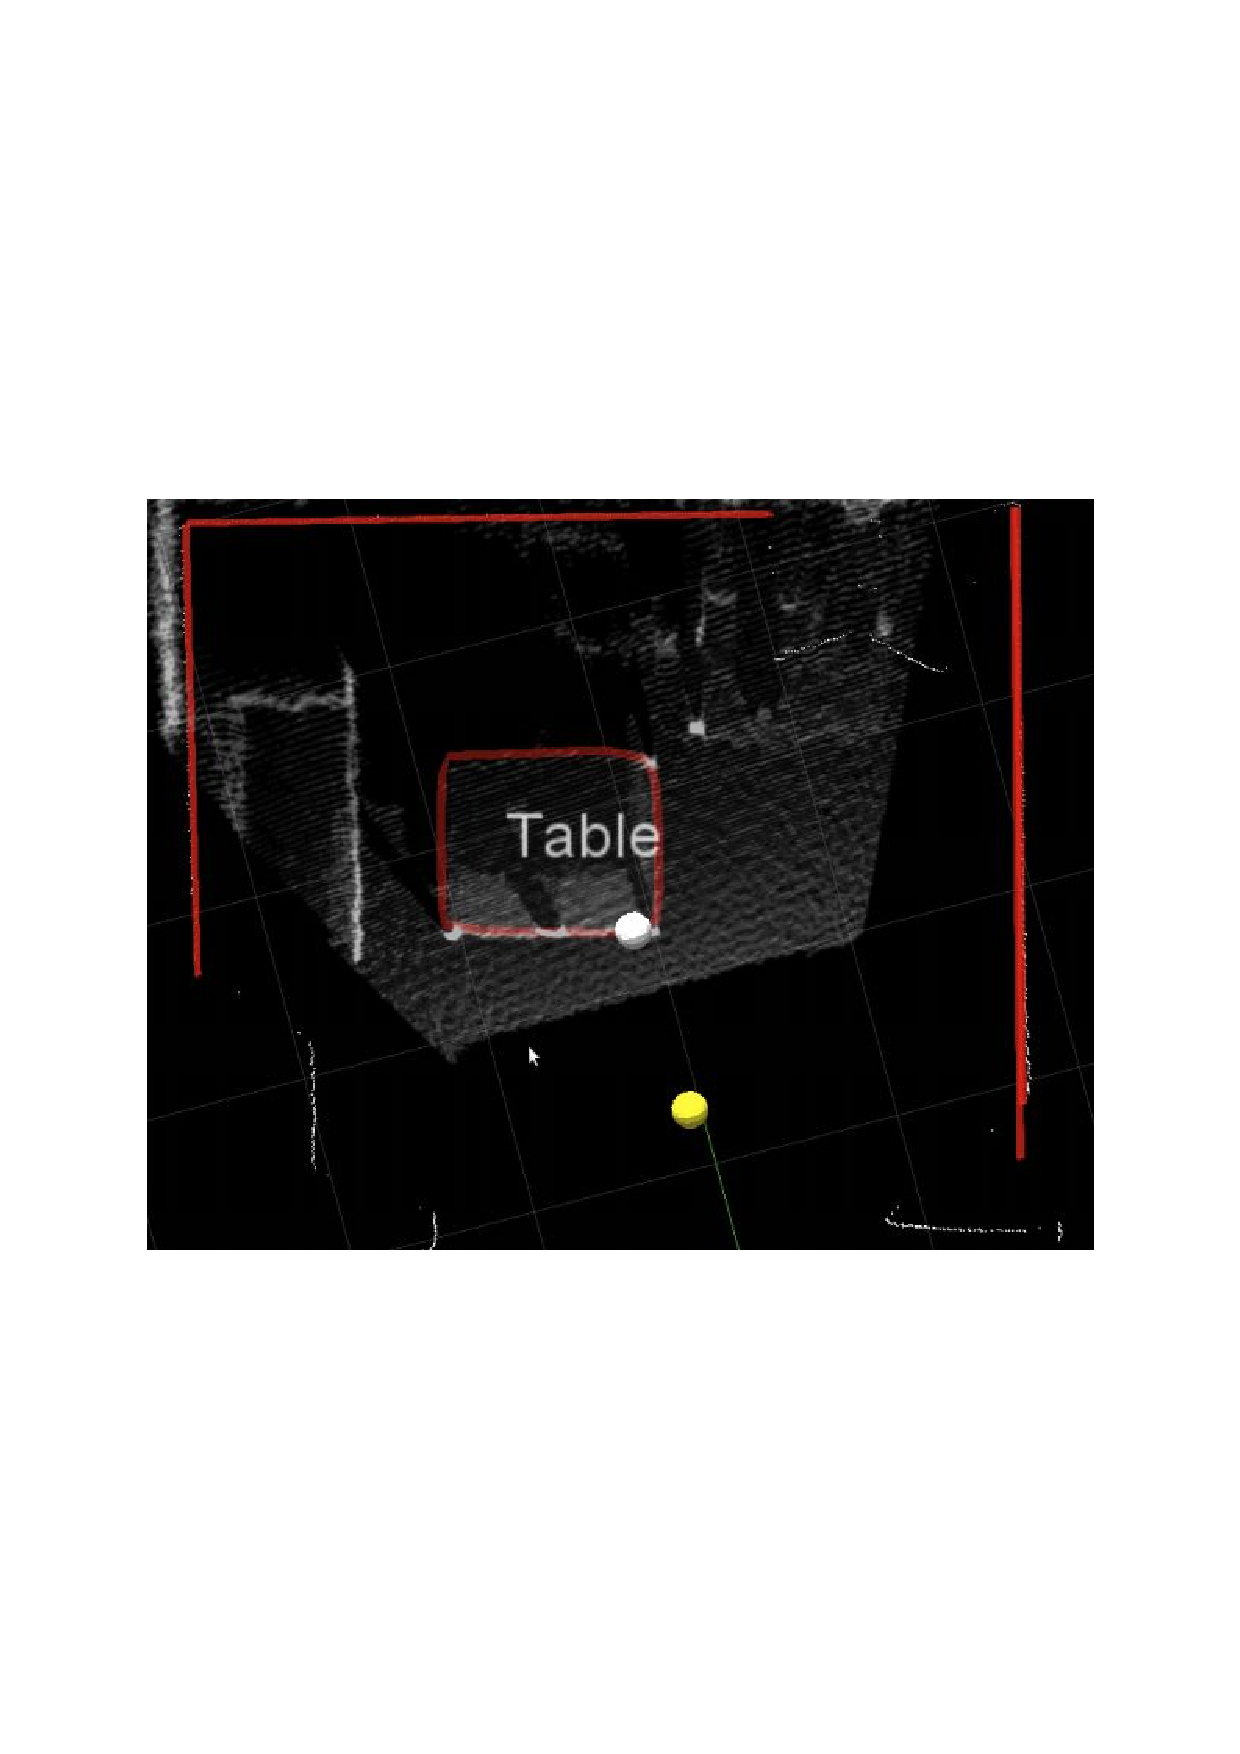
\includegraphics[width=0.44\textwidth]{pics/single_plane}
        }%
        \subfigure[]{%
           \label{fig:double_plane}
           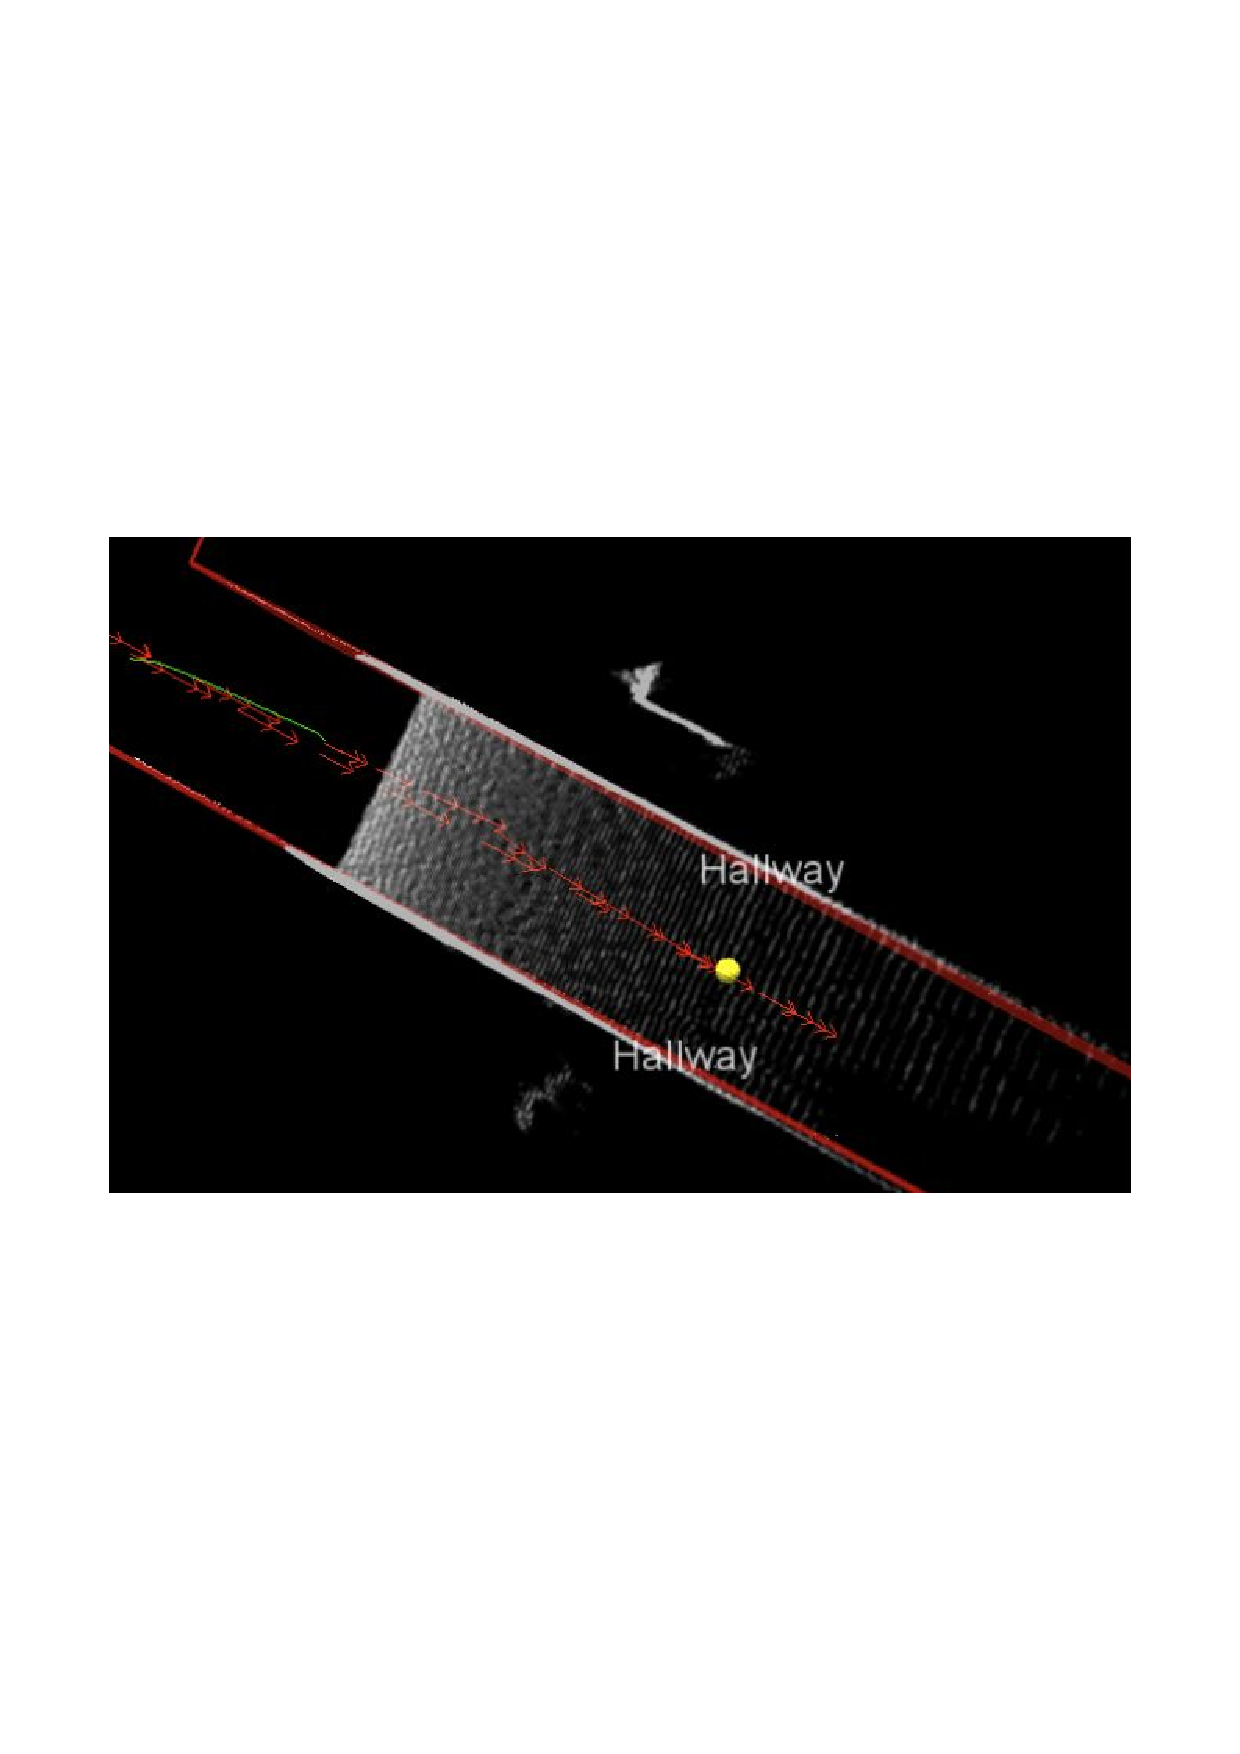
\includegraphics[width=0.54\textwidth]{pics/double_plane}
        } 
\caption{a) Top down point cloud view of a room. A planar landmark with label $Table$ has previously been annotated by a user. The convex hull for the planar landmark is shown in red lines. When asked to navigate to $Table$, the robot calculates a goal position, which is shown as the yellow point. b) Top down point cloud view of a hallway. The user has previously annotated two planar landmarks with the same label, $Hallway$. When asked to navigate to $Hallway$, the robot chooses a goal position in the middle of the planar landmarks, shown as the yellow point.}
\label{fig:navigation_plane_examples}
\end{figure}

When there are multiple planes associated with the same label, then we interpret this landmark as a region or space, such as a room or corridor. In this case, we project the points of all planes with this label to the ground plane, and compute the convex hull. The goal position is chosen as the centroid of the convex hull and goal orientation is unspecified, meaning the robot would not change its orientation upon reaching the goal position. An example goal position where the goal landmark label ''hallway" represents two walls enclosing a hallway is shown in Figure \ref{fig:double_plane}.

\subsubsection{Human-Aware Path Planning}
\label{sec:human_aware_path_planning}

After a goal position is calculated, a socially acceptable path is planned starting from the current position of the robot. Most approaches divide the robot path planning problem into two: global and local planning. Our approach adopts this template, and further divides global planning into two parts: static and dynamic planners. Static planner finds a path on the map of the environment by considering the safety, disturbance of humans and path length and but doesn't consider the future movements of humans. Dynamic planner simulates the reaction of humans and refines the static path. Dynamic planner takes the static path and refines it by considering the predicted temporary goals of humans, reaction to the robot's future movements. Our local planner is essentially a trajectory planner that computes the linear and angular velocities that would allow the robot to follow the dynamic path. The navigation system overview is shown in Figure~\ref{fig:navigation_overview}.

\begin{figure}[ht!]
\centering
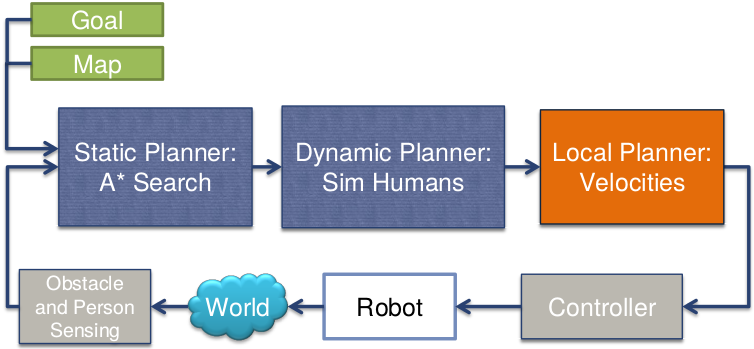
\includegraphics[width=0.55\textwidth]{pics/overview_crop.png}
\caption{System overview. When a map and goal is provided to the static planner, obstacles and humans are detected, then a path is planned using A* search. Dynamic planner refines the static plan by simulating human reactions to robot motion. Local planner receives the result, and computes the linear and angular velocities necessary to follow the path. The controller applies these velocities to the robot, which in turn acts in the world.}
\label{fig:navigation_overview}
\end{figure}


Static planner takes the start and goal positions and a 2D grid map as input and aims to find a set of waypoints that connects the start and goal cells. The output path has the minimum cost with regards to a linearly weighted cost function with 3 components: path length, safety and disturbance. We use A* search with Euclidean heuristics on a 8-connected grid map to find the minimum cost path. The path length cost is the total length of a path. The safety cost aims to model personal spaces of people. A gaussian cost function is attached to each person in the environment. The safety cost of a cell is the maximum safety cost value among all humans in the environment. Disturbance cost aims to represent the cases where the robot potentially disturbs the interaction of a group of humans. For example, if two people are facing each other and talking, then the robot should not cross between them. Disturbance cost is a non-zero cost if the robot's path crosses between two people who are in reasonable proximity to each other. We do not detect if there actually is conversation between the people, but estimate the disturbance cost using body poses of agents. This cost increases if body orientations of two people are facing each other and is inversely proportional on the distance between a pair of humans. 

The dynamic path refinement processes the static plan by simulating parts of the path where group of humans are closeby. We use Social Forces Model (SFM) \cite{helbing1995social} to simulate the motions of humans and the robot. Interaction between people are modeled as attractive and repulsive forces in SFM, similar to potential fields. The forces are recomputed iteratively and the resulting simulated paths replaces the corresponding path sections in the static plan. We use DWA as the local trajectory planner. The refinement steps allows considering future motions of humans due to the robot's future motions.

We demonstrate our approach with an example in simulation (Figure~\ref{fig:sim}). The goal of the robot is to navigate to a goal position in an office environment where there are 4 people present in the environment. In this scenario, we show how the path changes significantly when only poses of humans are varied. There are 3 main ways the robot can navigate to its goal: left, center or right corridor.

\begin{figure}[ht!]
\centering
%
        \subfigure[]{%
            \label{fig:sim2}
            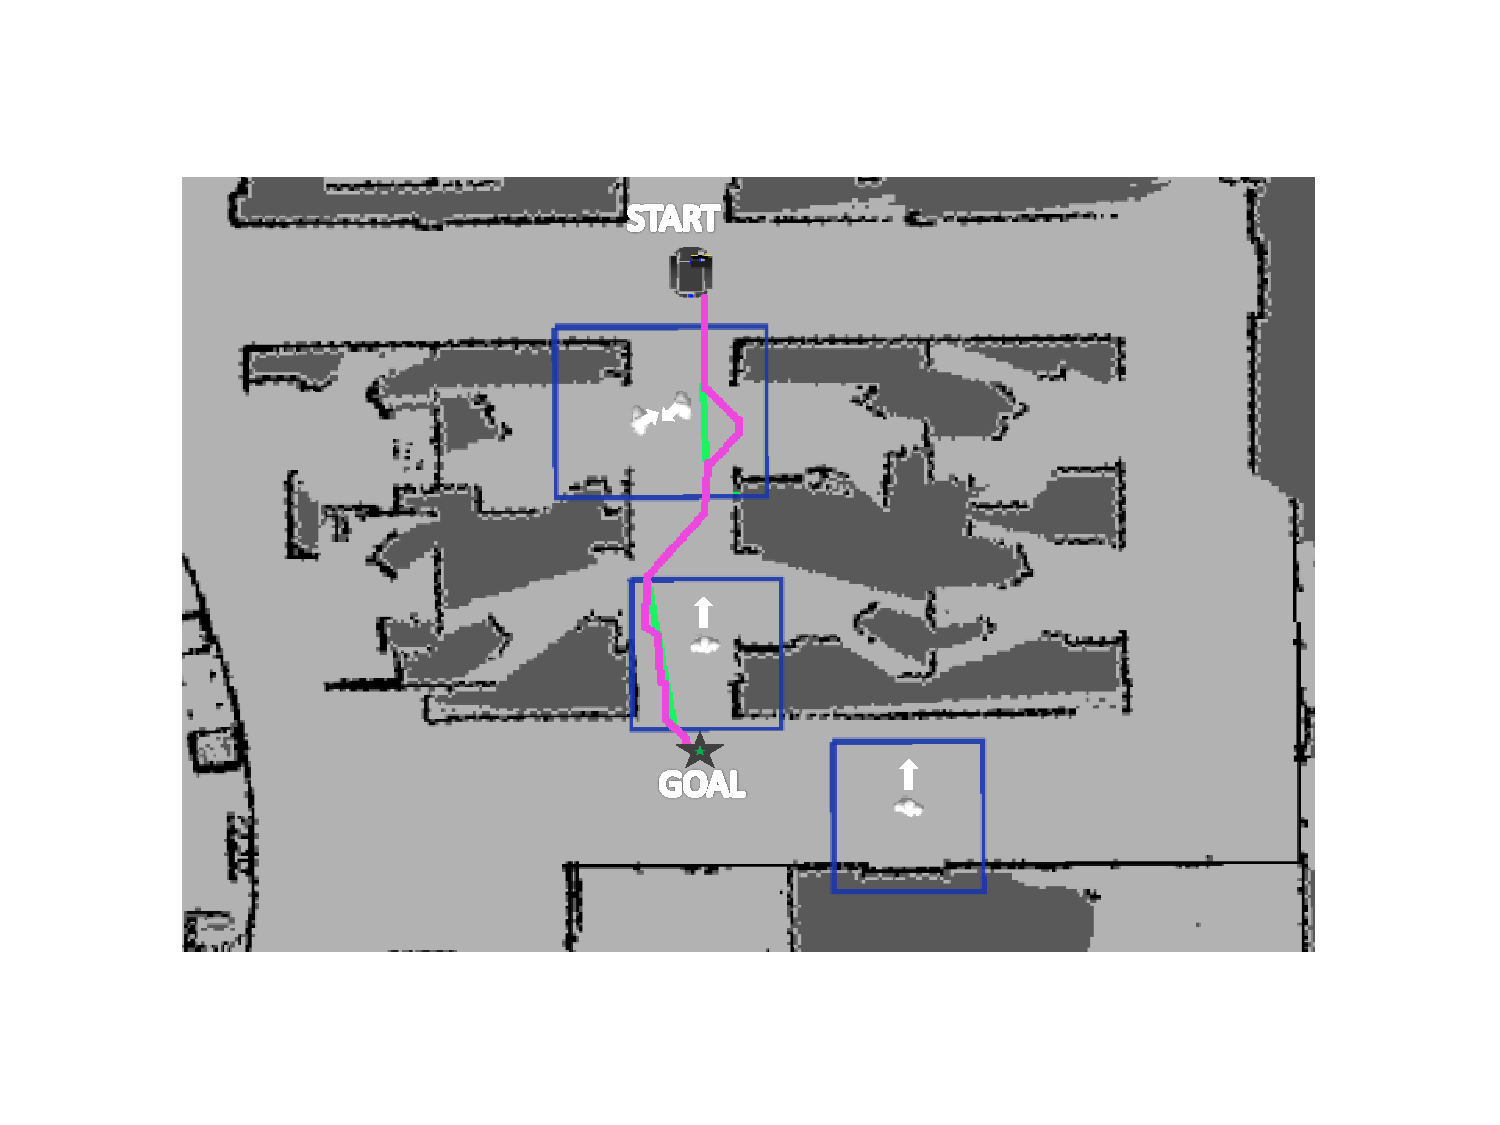
\includegraphics[width=0.4\columnwidth]{pics/sim2_crop}
        } 
        \subfigure[]{%
           \label{fig:sim3}
           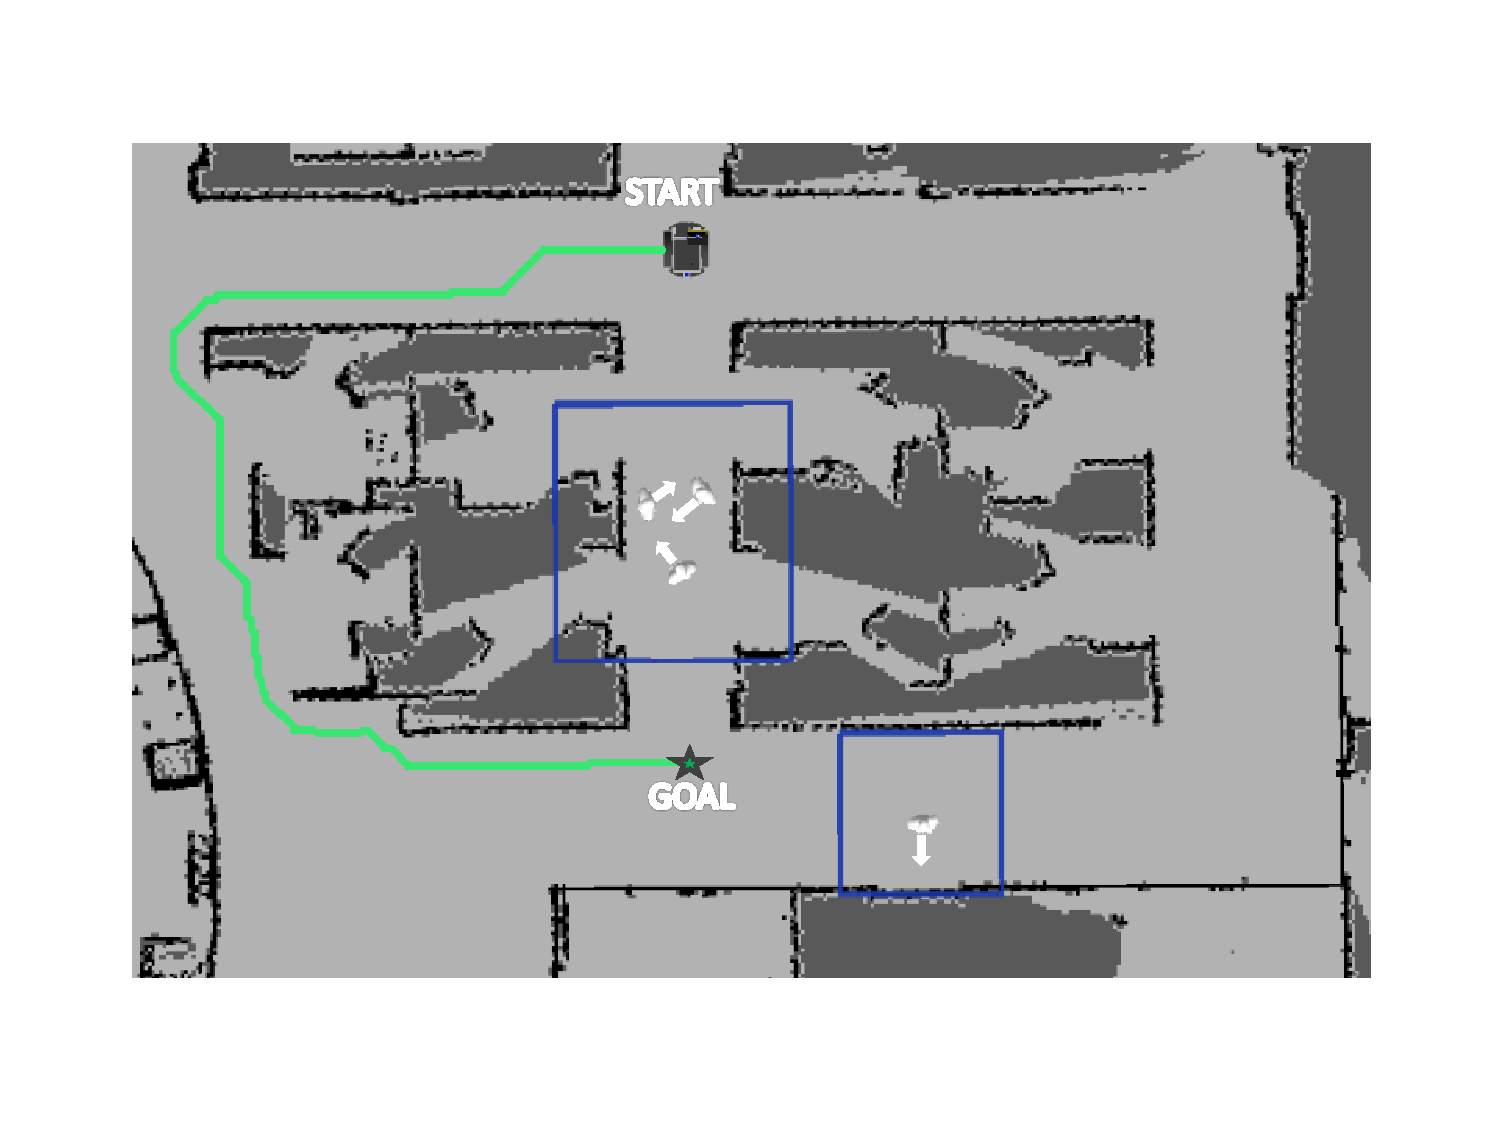
\includegraphics[width=0.4\columnwidth]{pics/sim3_crop}
        } \\
	\subfigure[]{%
           \label{fig:sim1}
           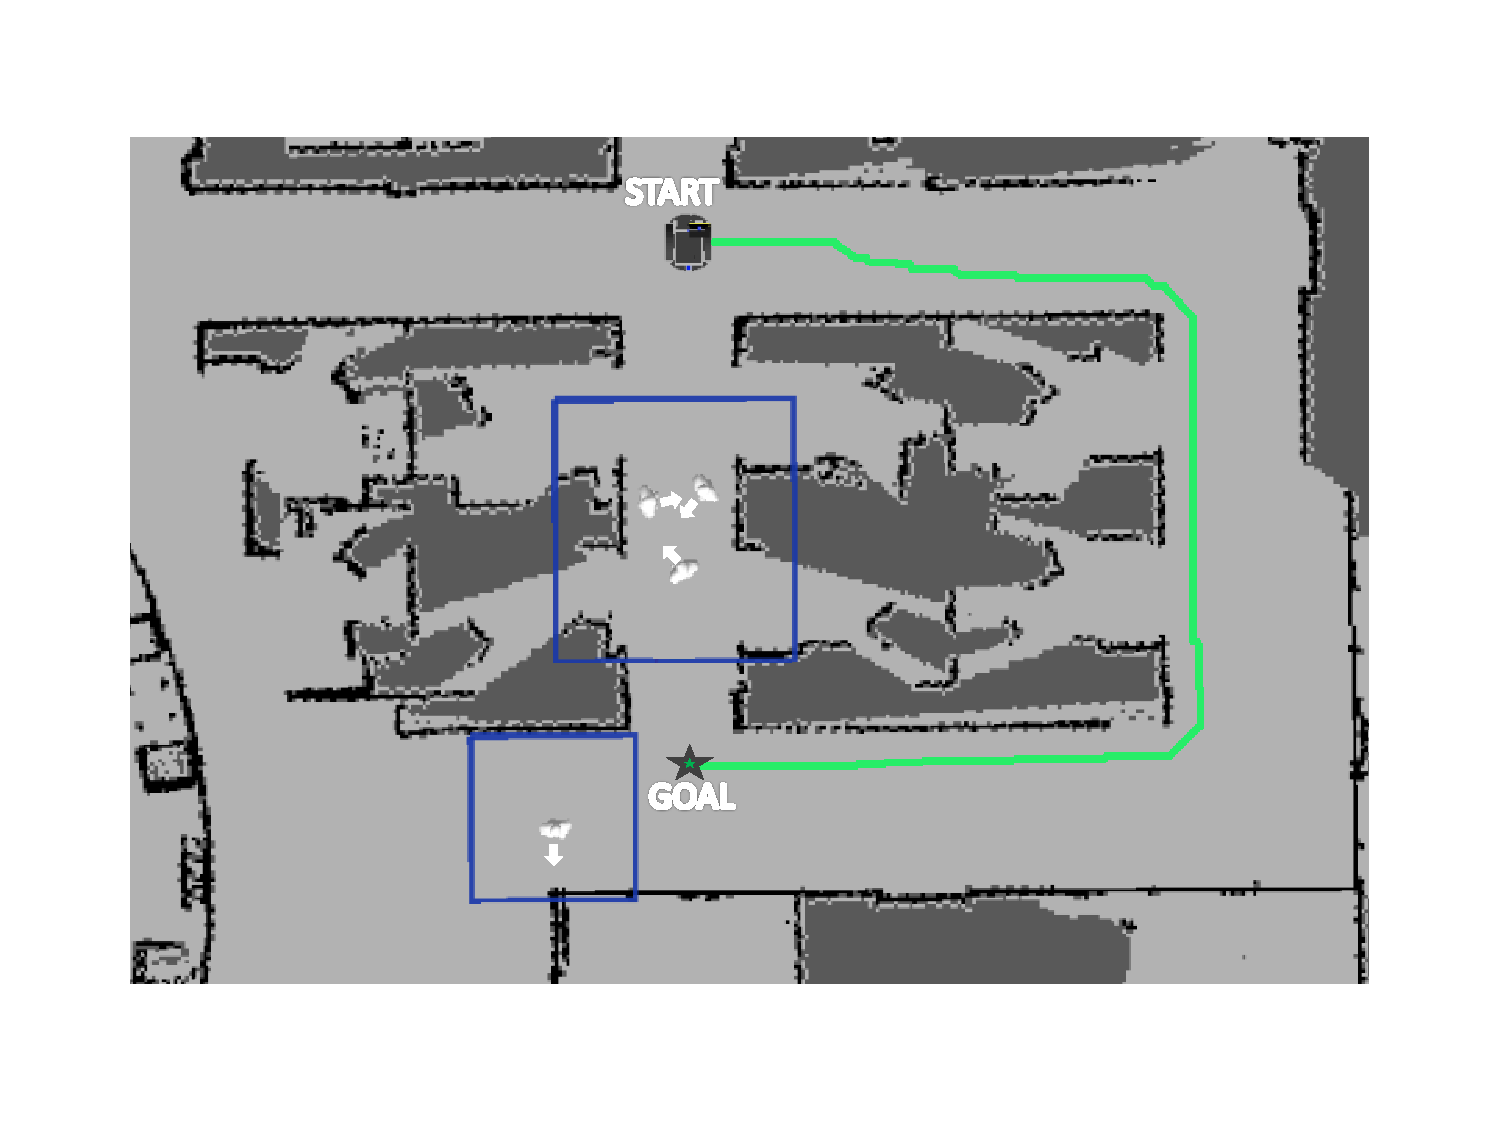
\includegraphics[width=0.4\columnwidth]{pics/sim1_crop}
        }
        
    \caption{%
	Path planner's output differ given the poses and grouping of humans. a) The robot takes shortest route, traveling in the vicinity of a group of two and another individual. b) third individual joins the group. Robot takes a longer path that doesn't have humans on path. c) fourth person changes his position, leading the robot to take the longest route.
     }%
   \label{fig:sim}
\end{figure}



In the first configuration in Figure~\ref{fig:sim2}, two people are grouped together as they are looking at each other and likely conversing. The robot decides to take the center corridor, first slightly disturbing the speaking duo, then switches sides in the corridor and reaches its goal. In the figure, the dynamic path (pink line) is overlaid on the static path (green line). 

In the second configuration in Figure~\ref{fig:sim3}, The third person at the center corridor joins the conversation. Now we have 2 group regions (rectangles) in the scene. Since passing through a group of 3 people would introduce a high disturbance cost in addition to the safety cost, the robot decides to take a longer route (left corridor). Since this path does not intersect any group regions, dynamic simulation was not conducted.

In the third configuration in Figure~\ref{fig:sim1}, the group of three hasn't moved, but the fourth person person has changed its position. In this case, if the left corridor is taken again, an additional safety cost would be incurred. Therefore the robot decides to take the longest route (right corridor). Again, since the robot travels far from humans, dynamic simulation was not conducted.

\subsection{Context-Aware Person Following}
\label{sec:context_aware_person_following}

As briefly reviewed in Section \ref{sec:rel_context_aware_navigation}, most person following methods in the literature have the same underlying principle: a target position is calculated given the human's position and a control method finds actions iteratively to navigate toward the target positions. This results in reactive robot behaviors where the robot follows the human blindly, irrespective of the task and context. Our person following method presented in Section \ref{sec:person_following} also falls under this category.

Although reactive methods are sufficient for some scenarios, it can easily lead to deadlock scenarios. For example, consider the case that the followed person goes through a door and stops just outside the doorway. In this case, the robot would occupy the doorway, blocking other people's passage, however does not know it caused an undesirable social situation. If the robot knows what the user intends to do, it can anticipate those actions and suitably adjust its behavior. Person following can be used in different contexts, such as for carrying luggage in airports or groceries in a supermarket. We showed in previous sections that semantic information could be used to communicate goals between the robot and the user. The stored semantic information can also be used to facilitate robot navigation.

We model the task scenario during person following as a state machine, where transitions are triggered via events. A general scenario during person following is implemented as a sequence of four phases:

\begin{enumerate}
\item Signal: Robot detects an event using perceptual cues
\item Approach: Robot moves to a position better suited to the task
\item Execution: Robot and/or Human execute the task
\item Release: Robot detects the end of event and continues with the basic following behavior
\end{enumerate}

We focus on two specific scenarios of context-aware person following, using the 4-phase model: following for labeling in Section \ref{sec:following_for labeling} and passing doors in Section \ref{sec:following_door_passing}.

\subsubsection{Following for Interactive Labeling}
\label{sec:following_for labeling}

We first examine person following scenario for interactive labeling of semantic landmarks, as described in Section \ref{sec:interactive_map_labeling}. For this scenario the robot follows the user as he/she moves between the landmarks or objects of interests. Sometimes when a user wants to label an object, undesirable social situations can occur because the robot does not have the task context. In this example, the context is defined as the understanding of being a part of a collaborative task: interactive labeling. When a user stops in front of a landmark or object to label it, if the robot stays behind, it can not perceive the pointing gesture and the landmark at the same time. This situation is illustrated in Figure \ref{fig:landmark_labeling_example}. 



\begin{figure}[ht!]
\centering
        \subfigure[]{%           
           \label{fig:label_ex_1}
           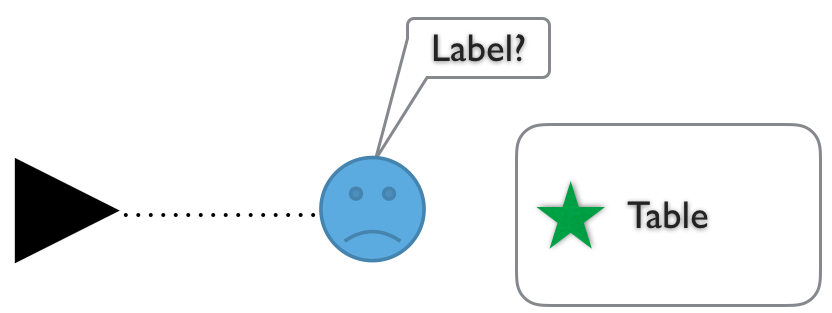
\includegraphics[width=0.3915\textwidth]{pics/label_ex_1}
        }
         \subfigure[]{%           
           \label{fig:label_ex_2}
           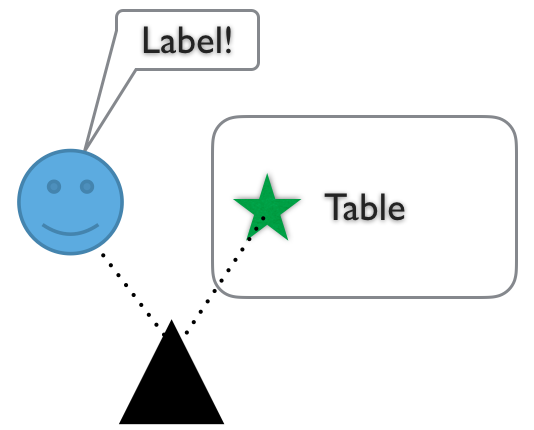
\includegraphics[width=0.2565\textwidth]{pics/label_ex_2}
        } 
    \caption{a) A common problem encountered during person following for interactive labeling. The user wants to label an object on the table, however the robot does not know the user's intention and stays behind at a fixed distance to the user. b) Our solution is for the robot to navigate to a location that gives the robot a better chance to observe the user and the object simultaneously.}
   \label{fig:landmark_labeling_example}
\end{figure}


The robot can behave more intelligently if the robot can predict ahead of time when the user is going to label a landmark. When the robot detects that the user intends to label a landmark or object, our approach is to position the robot base so it has a better chance to perceive both the pointing gesture and the object/landmark of interest. 


\begin{figure}[h]
\centering
%
        \subfigure[]{%           
           \label{fig:situtation_aware_landmark_labeling0}
           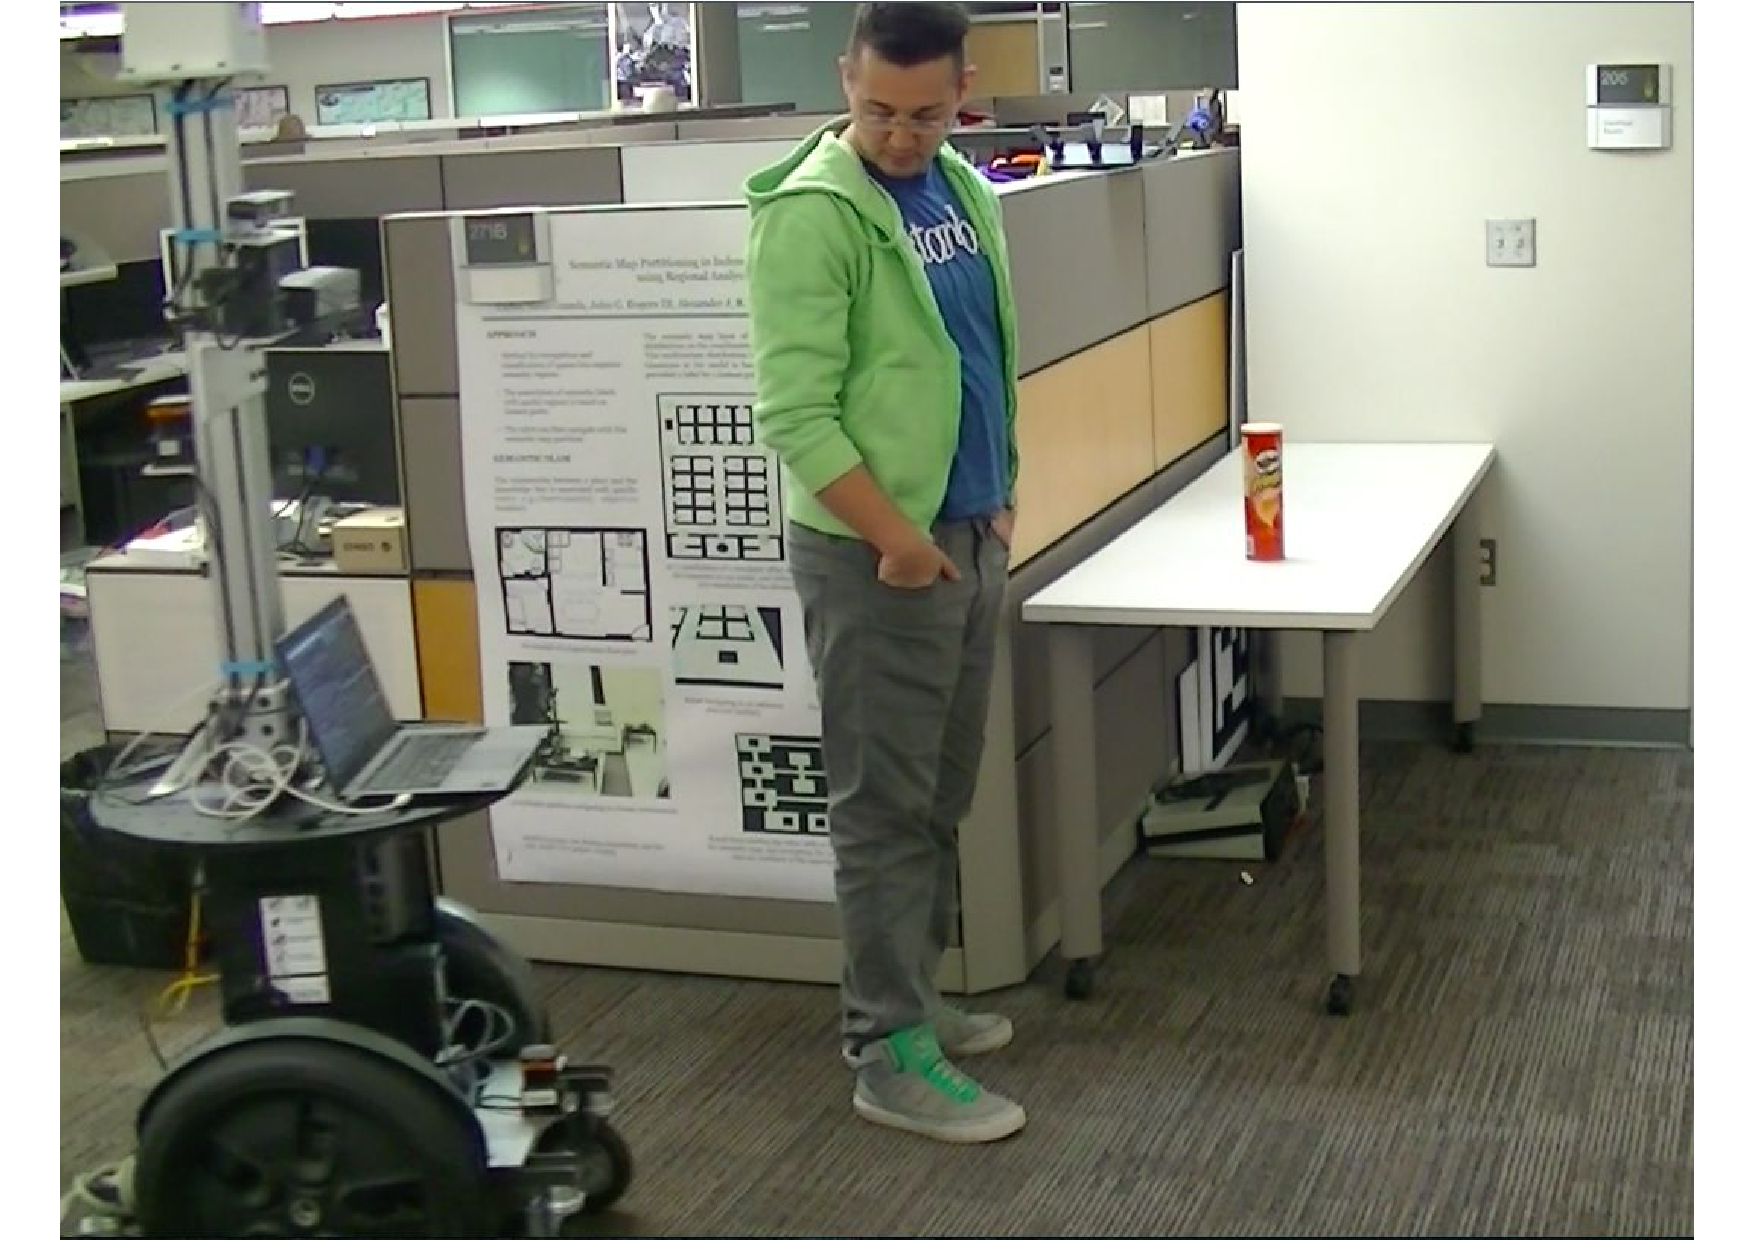
\includegraphics[width=0.445\textwidth]{pics/sit_table_00}
        } 
         \subfigure[]{%           
           \label{fig:situtation_aware_landmark_labeling2}
           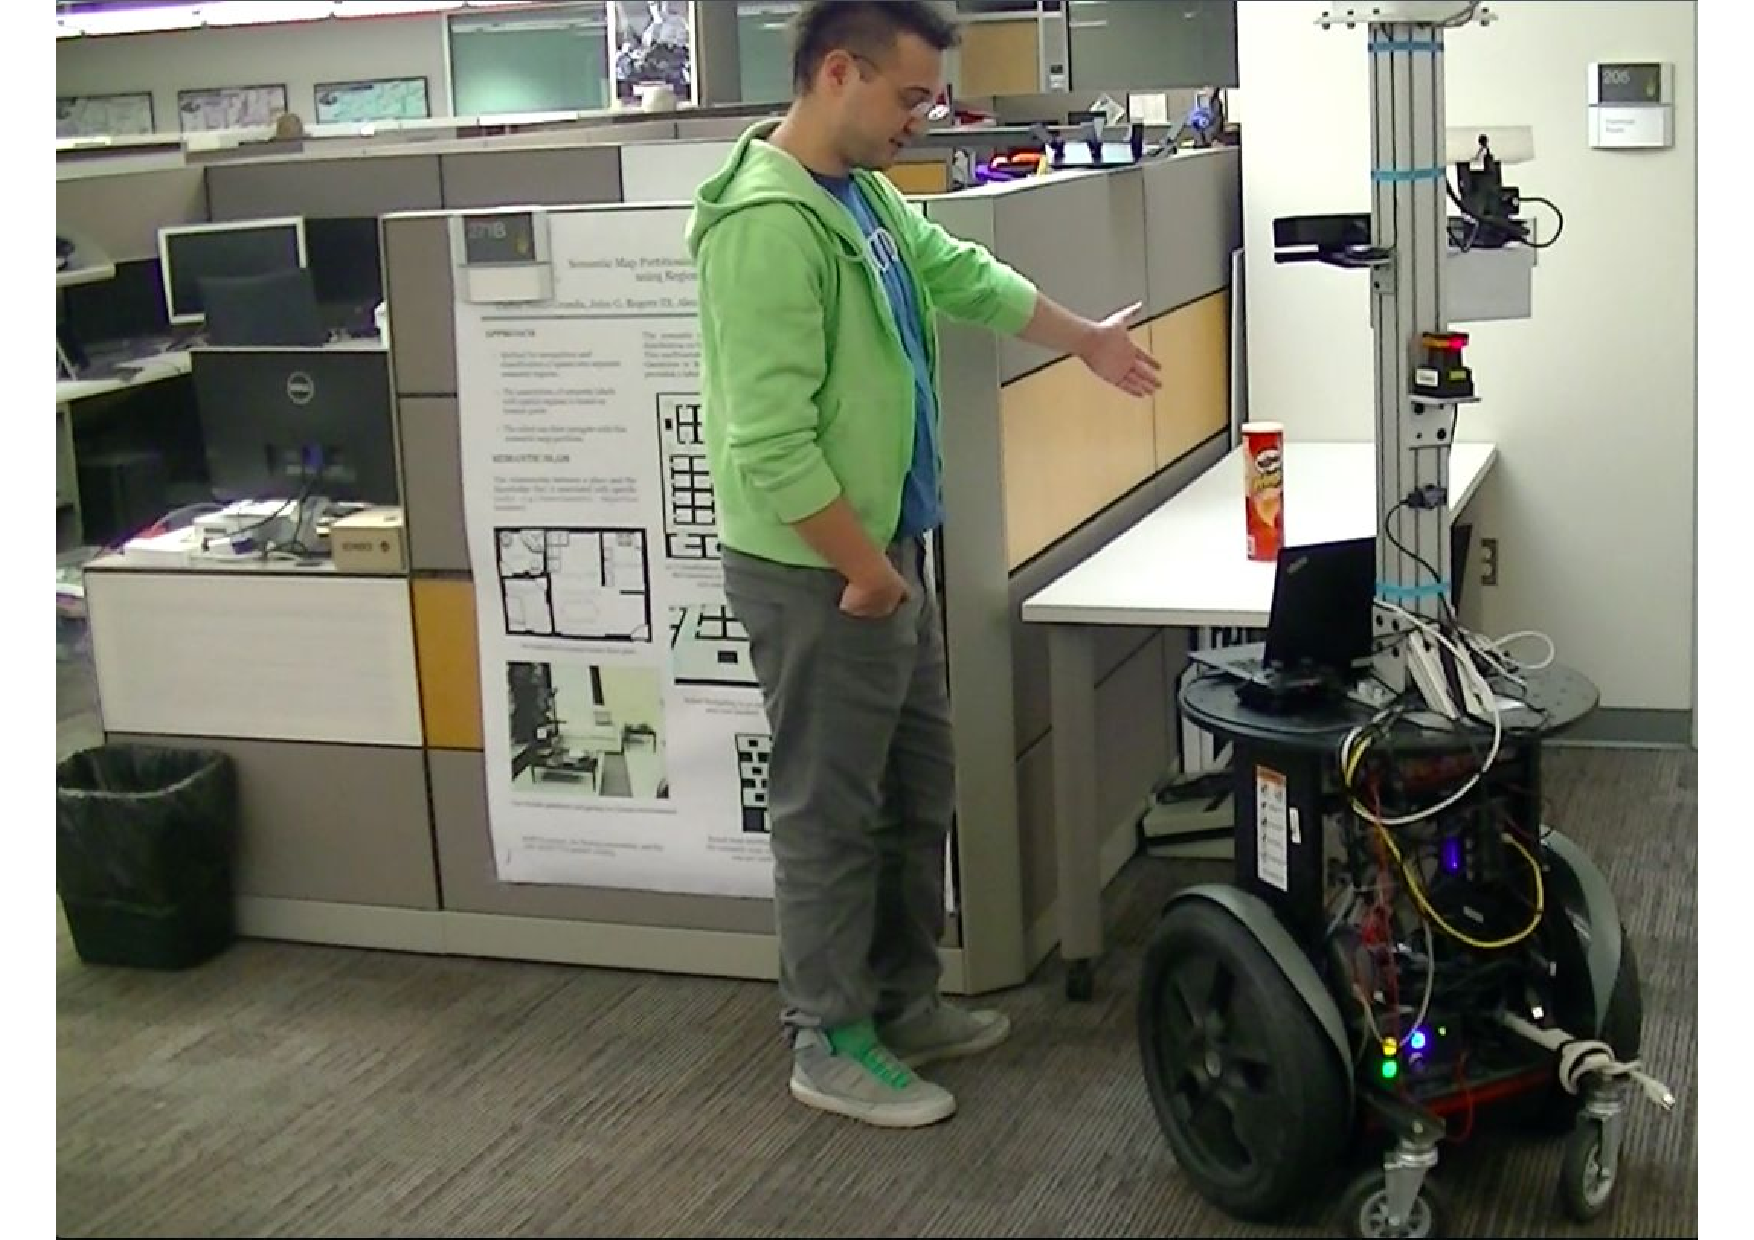
\includegraphics[width=0.45\textwidth]{pics/sit_table_02}
        } \\
        \subfigure[]{%
        	\label{fig:situtation_aware_landmark_labeling3}
            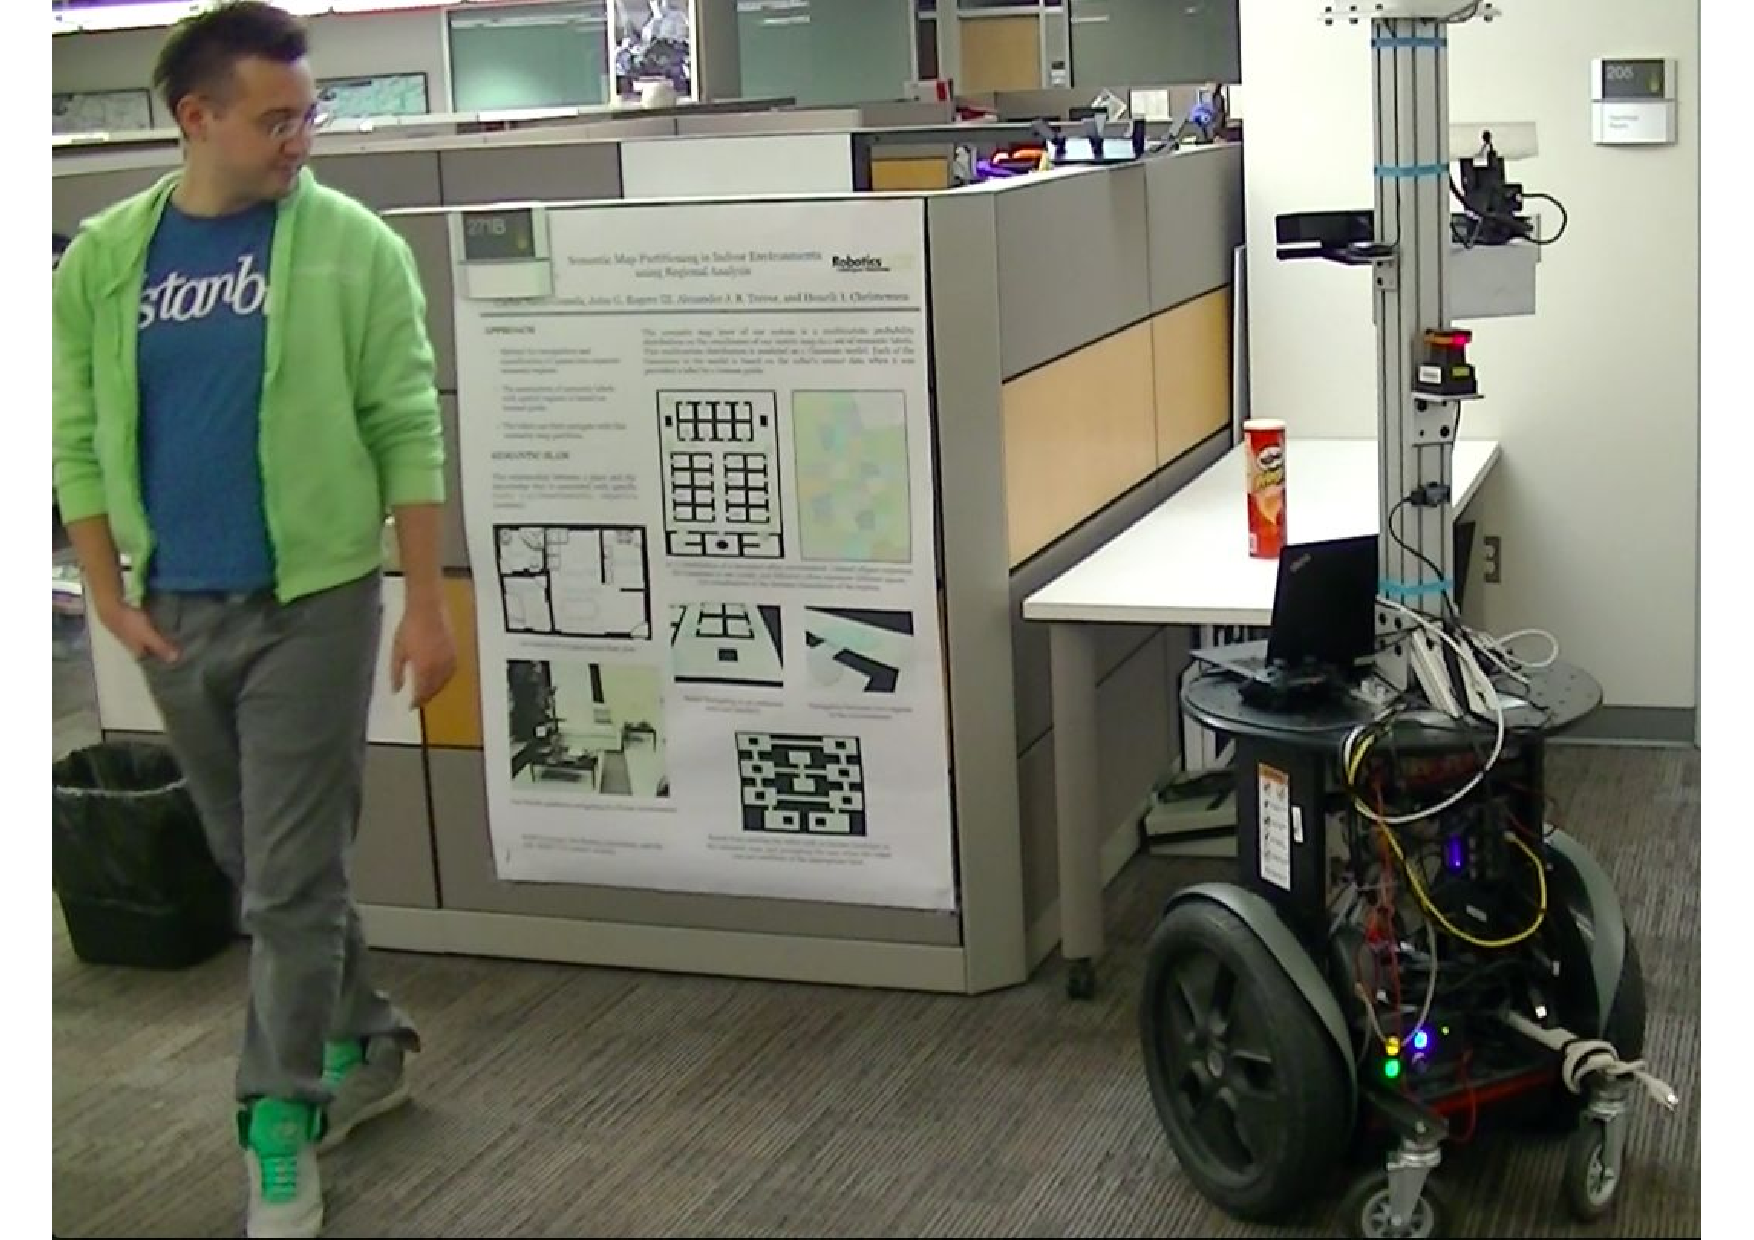
\includegraphics[width=0.45\textwidth]{pics/sit_table_03}
        }%\\        
        \subfigure[]{%           
           \label{fig:situtation_aware_landmark_labeling4}
           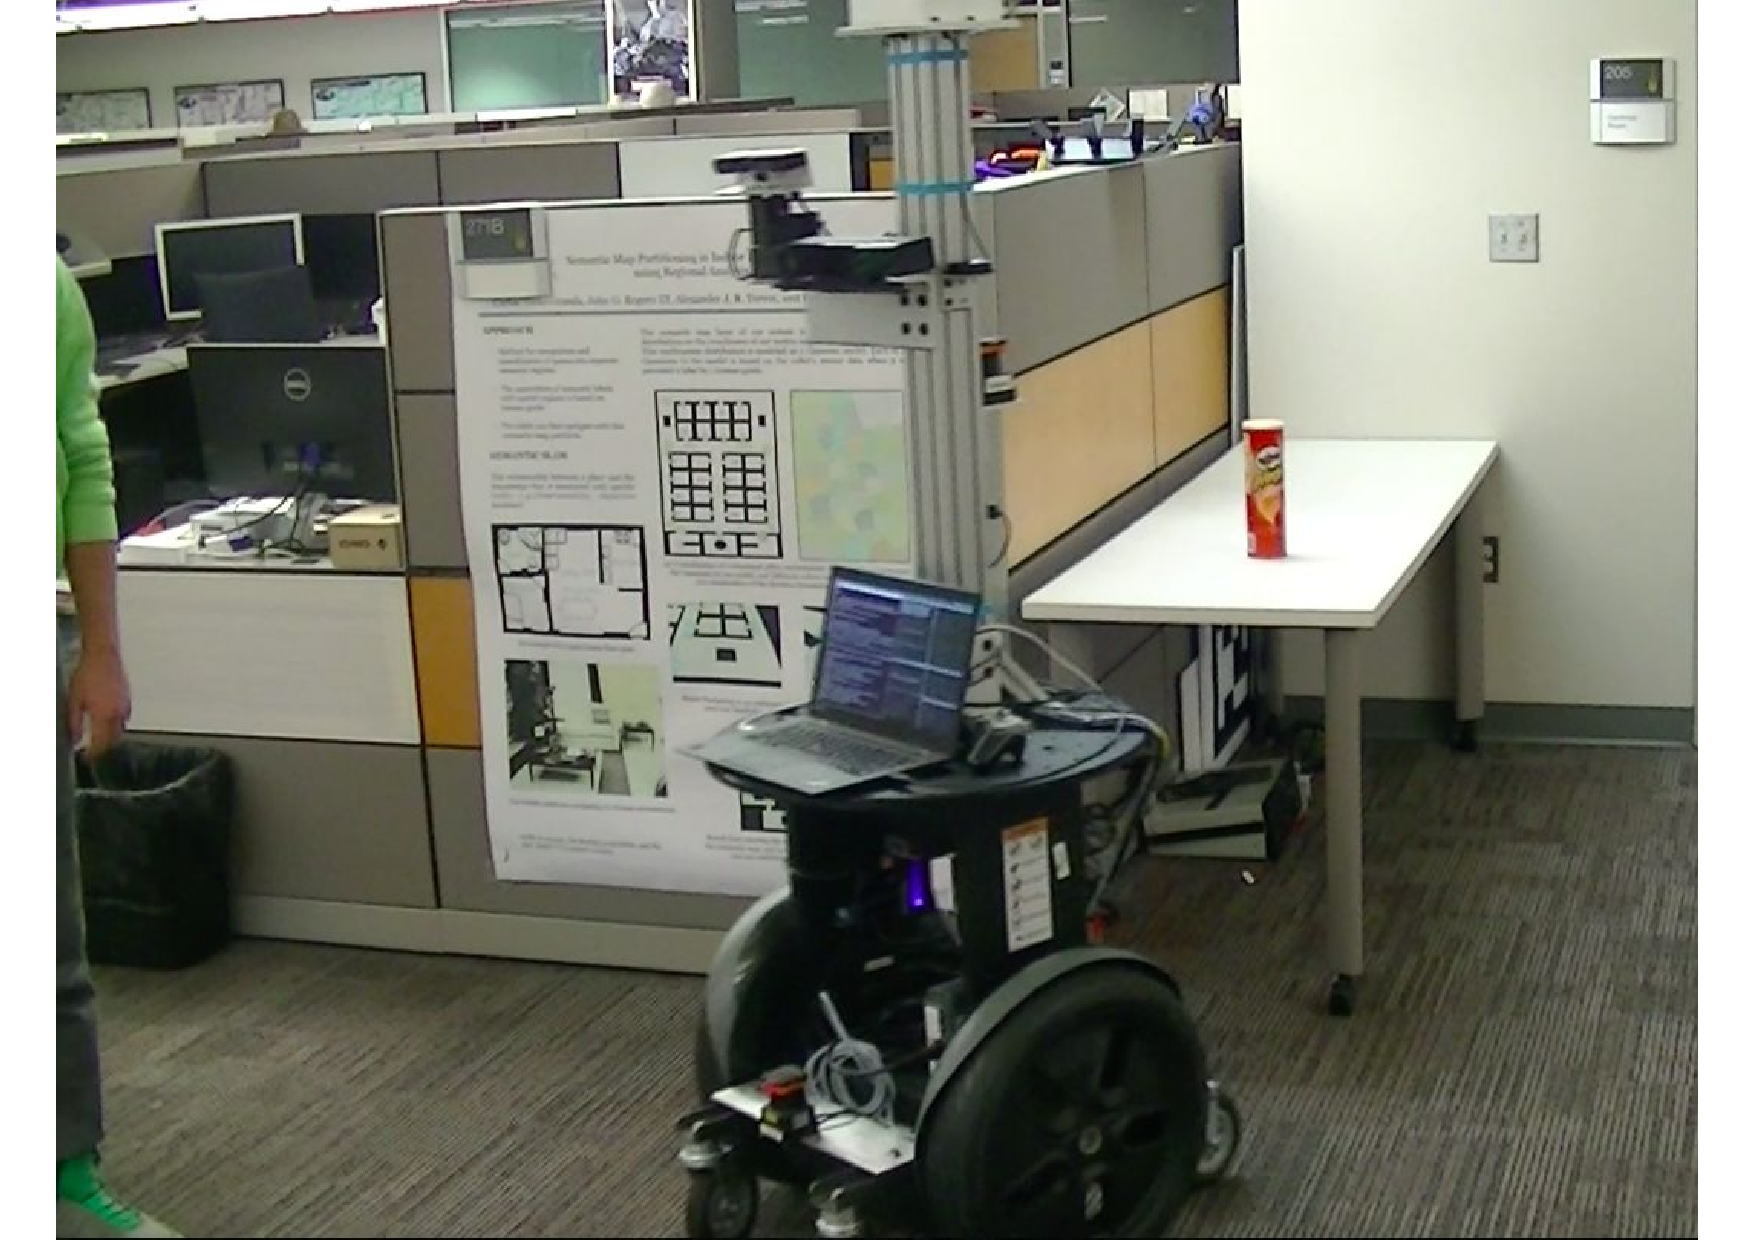
\includegraphics[width=0.46\textwidth]{pics/sit_table_04}
        }
    \caption{Demonstration of context-awareness for interactive labeling. The robot is following the user throughout the environment and keeping a fixed distance of $1.2m$ to the user. a) Signal phase: The user has stopped and is in the cloxe proximity to the convex hull of the table. b) Approach phase: The robot calculates and navigates to a goal position, so it can perceive the pointing gesture and target. Execution phase: The user points out to the object on the table. c) Release phase: user moves away from the table d) Basic following behavior continues.}
   \label{fig:situtation_aware_landmark_labeling}
\end{figure}

We follow the 4-phase behavior design for person following for interactive labeling. The Signaling phase is triggered whenever the user is close to a unlabeled landmark in the semantic map. The user must have close to zero speed to enable signaling for this behavior, because the user may walk past the landmark. After the robot detects the signal, we sample positions around the group to locate a ``suitable" goal pose for the robot. A pose that is collision free but that gives the robot highest chance of interaction is favored. A suitable goal position should be at equal distance to the landmark and the user, and goal orientation should be selected so the robot faces in between the landmark and the user. Moreover, the goal point should not be very close to an obstacle. We linearly sample points around the ''group" formed by the user and the landmark's centroid. The points are sampled from the \textit{p-space} of this group, which is a circle that includes the landmark and user center positions. This is influenced by Kendon's work \cite{kendon1990conducting} on how people form groups in interactive settings. Every sampled position $p$ has a score of:
\[
Score(p) = 1.0 - Cost_{visibility}(p) - Cost_{obstacle}(p)
\]
Where we define the costs as:
\begin{align} 
\begin{split}
Cost_{visibility}(p)&=dist(user,landmark)/(dist(p,landmark)-dist(p,user)) \\
Cost_{obstacle}(p)&=max(local\_cost(p),global\_cost(p))
\end{split}
\end{align}

The local and global costs are fetched from the normalized local costmap, which is formed by the laser scanner readings. The sample with the highest non-negative score is chosen as the goal position. The orientation of the robot is chosen as looking toward the center of all the people in the group. 

\begin{table}[ht!]

	\caption{Conditions to trigger phases when the user is involved with the Landmark Labeling Event during following.}
    \centering
		
  \begin{tabular}{l |  m{10cm}}
    \toprule    
    Signal & {$dist(user, convex hull(landmark))<threshold$}\\       
	                           & {$speed(user)\sim 0$} \\
	                           & {person roughly facing landmark}\\ \midrule		                           		                                
    Approach & {Optimal Goal: Close to both the landmark and person, facing in between}\\       \midrule
    Execution & {User points and labels landmark}\\  \midrule
    Release & {$dist(user, convex hull(landmark))>threshold$}\\ 
    \bottomrule
  \end{tabular}
    \label{table:situation_aware_list_landmark}
\end{table}

When the robot completes its move to the goal position, the user labels the landmark or objects via pointing gestures. After the task is completed, the robot waits until the user to leaves the vicinity of the landmark. When that happens, the robot continues following the user. If, during any of the phases, the person tracking fails, it informs the user so following can be restarted. The phases and conditions for this behavior are summarized in Table \ref{table:situation_aware_list_landmark}. Images from a demonstration for this behavior is shown in Figure \ref{fig:situtation_aware_landmark_labeling}.

\subsubsection{Door Passing}
\label{sec:following_door_passing}



The second behavior we inspect during person following is door passing. In our experience, the a reactive person following behavior can cause problems while passing doors. For example, if the user intends to close an open door or open a closed door, the robot might end up blocking the movement of the door. Moreover, a deadlock situation occurs when the user wants to go through a door with spring-loaded hinges. In that case, the user would need to hold to door to keep it open, and because the distance between the robot and the user is less than the following threshold, the robot would stay still and won't pass the door.

The robot can assume that the user might be intending to open, close or pass through a door when the user is approaching the door. In our approach, the robot continuously monitors user's proximity to the doors using the semantic map, if the door signs were detected and added to the semantic map beforehand, as explained in Section \ref{sec:door_signs}.

\begin{table}[ht!]
	\caption{Conditions to trigger phases when the user is passing through a door during following.}
	\centering
  \begin{tabular}{l |  m{10cm}}    
    \toprule    
    Signal & {$dist(user, convexhull(door))<threshold$}\\         
    	      & {$speed(user)\sim 0$} \\
	      & {User performs pointing gesture towards the passage}\\ \midrule	                           
    Approach & {Optimal Goal: A position on the other side of the door that doesn't block the doorway}\\       \midrule
    Execution & {Robot and user meet at the same side of the door}\\  \midrule
    Release & {$dist(user, convexhull(door))>threshold$ }\\ 
    \bottomrule
  \end{tabular}
    \label{table:situation_aware_list_door}
\end{table}

The phases and conditions for door passing situation are summarized in Table \ref{table:situation_aware_list_door}. The robot takes action when the user is nearby a door and performs a pointing gesture towards it, to signal that the robot should pass from the door (Signal Phase). If the action is not signaled, the robot continues with basic following during the door passage. After the detection of a pointing gesture, a goal position is calculated (Approach Phase). The goal positions are sampled on the other side of the door, that is guaranteed not the block the opening/closing of the door. A collision-free position with the least obstacle cost sample is chosen as the goal point. Note that while the robot is moving, it does not aim to keep fixed distance to the user anymore. After the robot reaches the goal, it waits for the person to pass the door (Execution Phase). After the user moved away from the door, the standard following behavior takes over. Images from the demonstration of context-aware person following for door passing is shown in Figure \ref{fig:situtation_aware_door_passing}.

\begin{figure}[ht!]
\centering
%
        \subfigure[]{%           
           \label{fig:situtation_aware_door_passing0}
           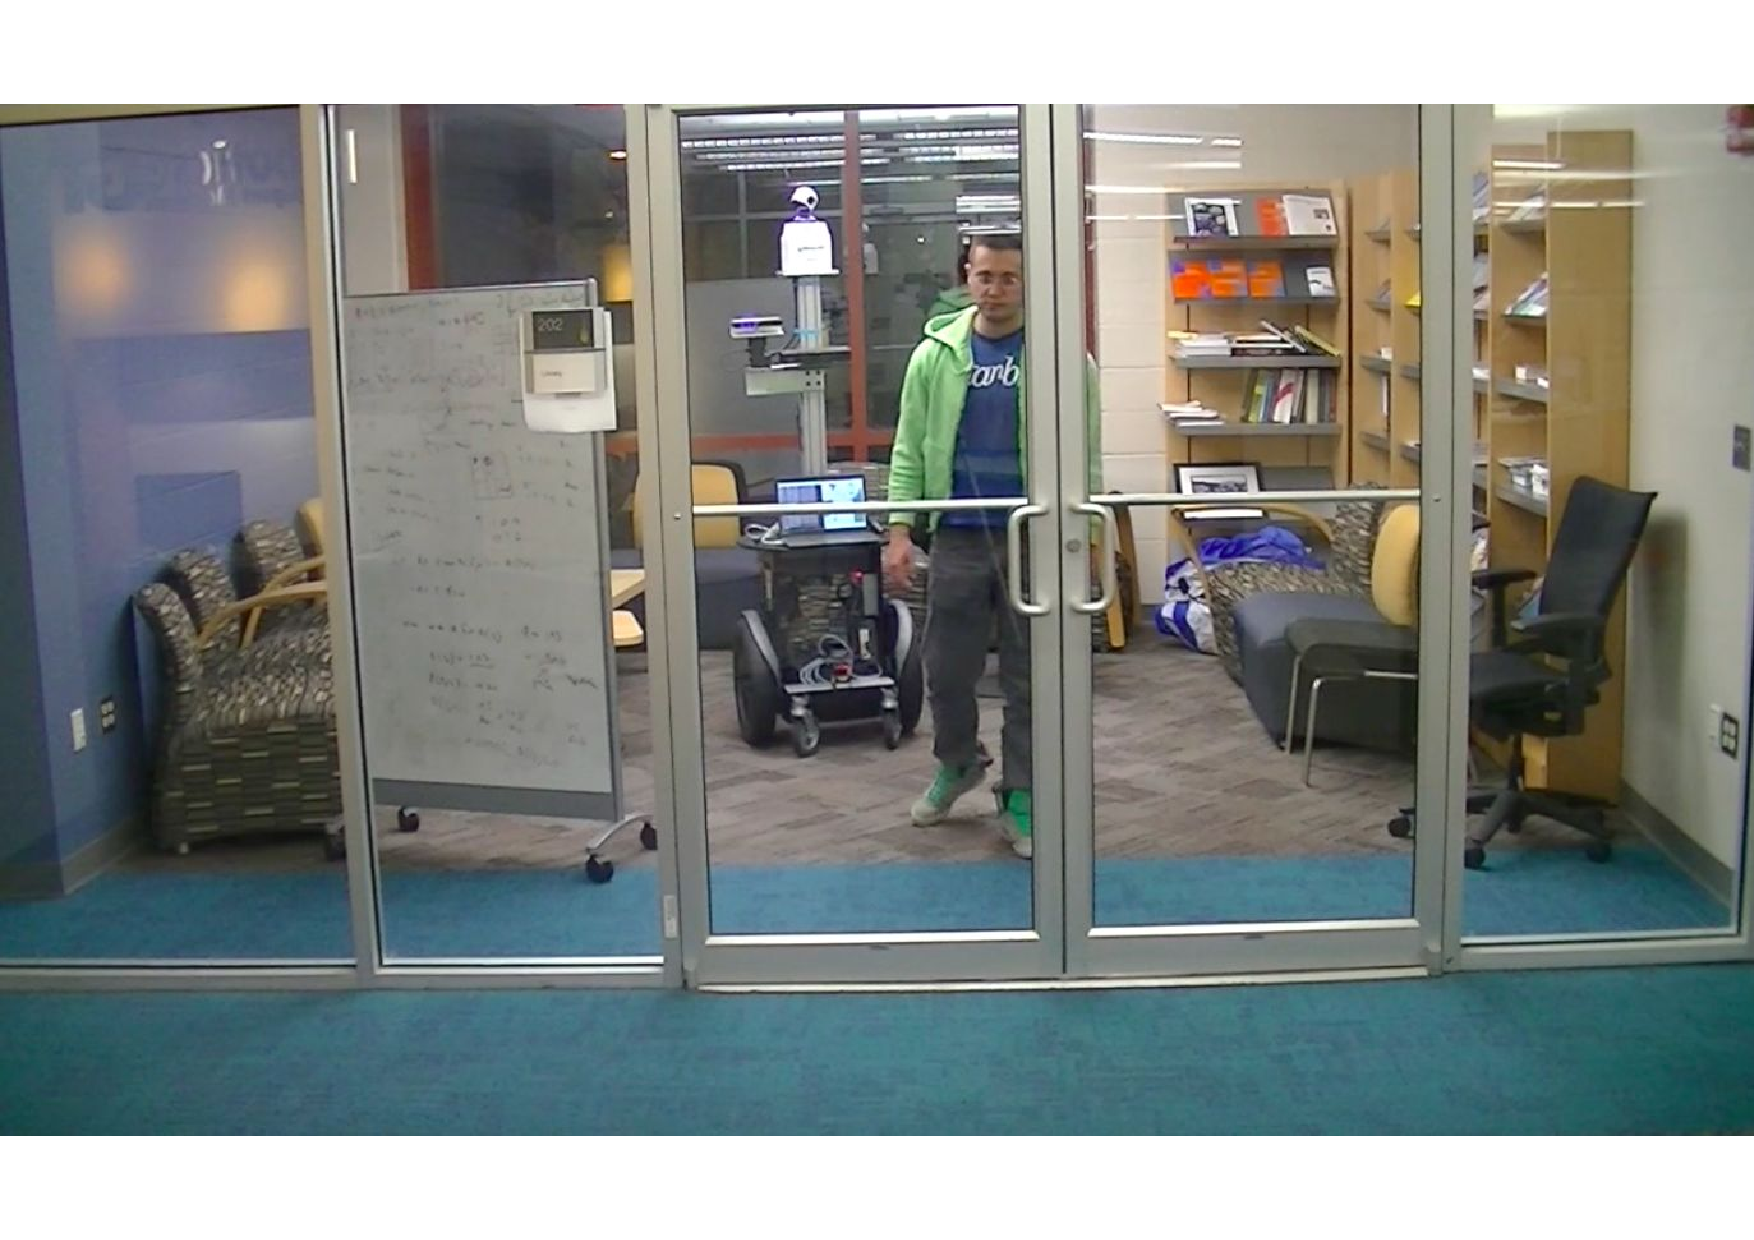
\includegraphics[width=0.445\textwidth]{pics/sit_door_00}
        } 
        \subfigure[]{%           
           \label{fig:situtation_aware_door_passing1}
           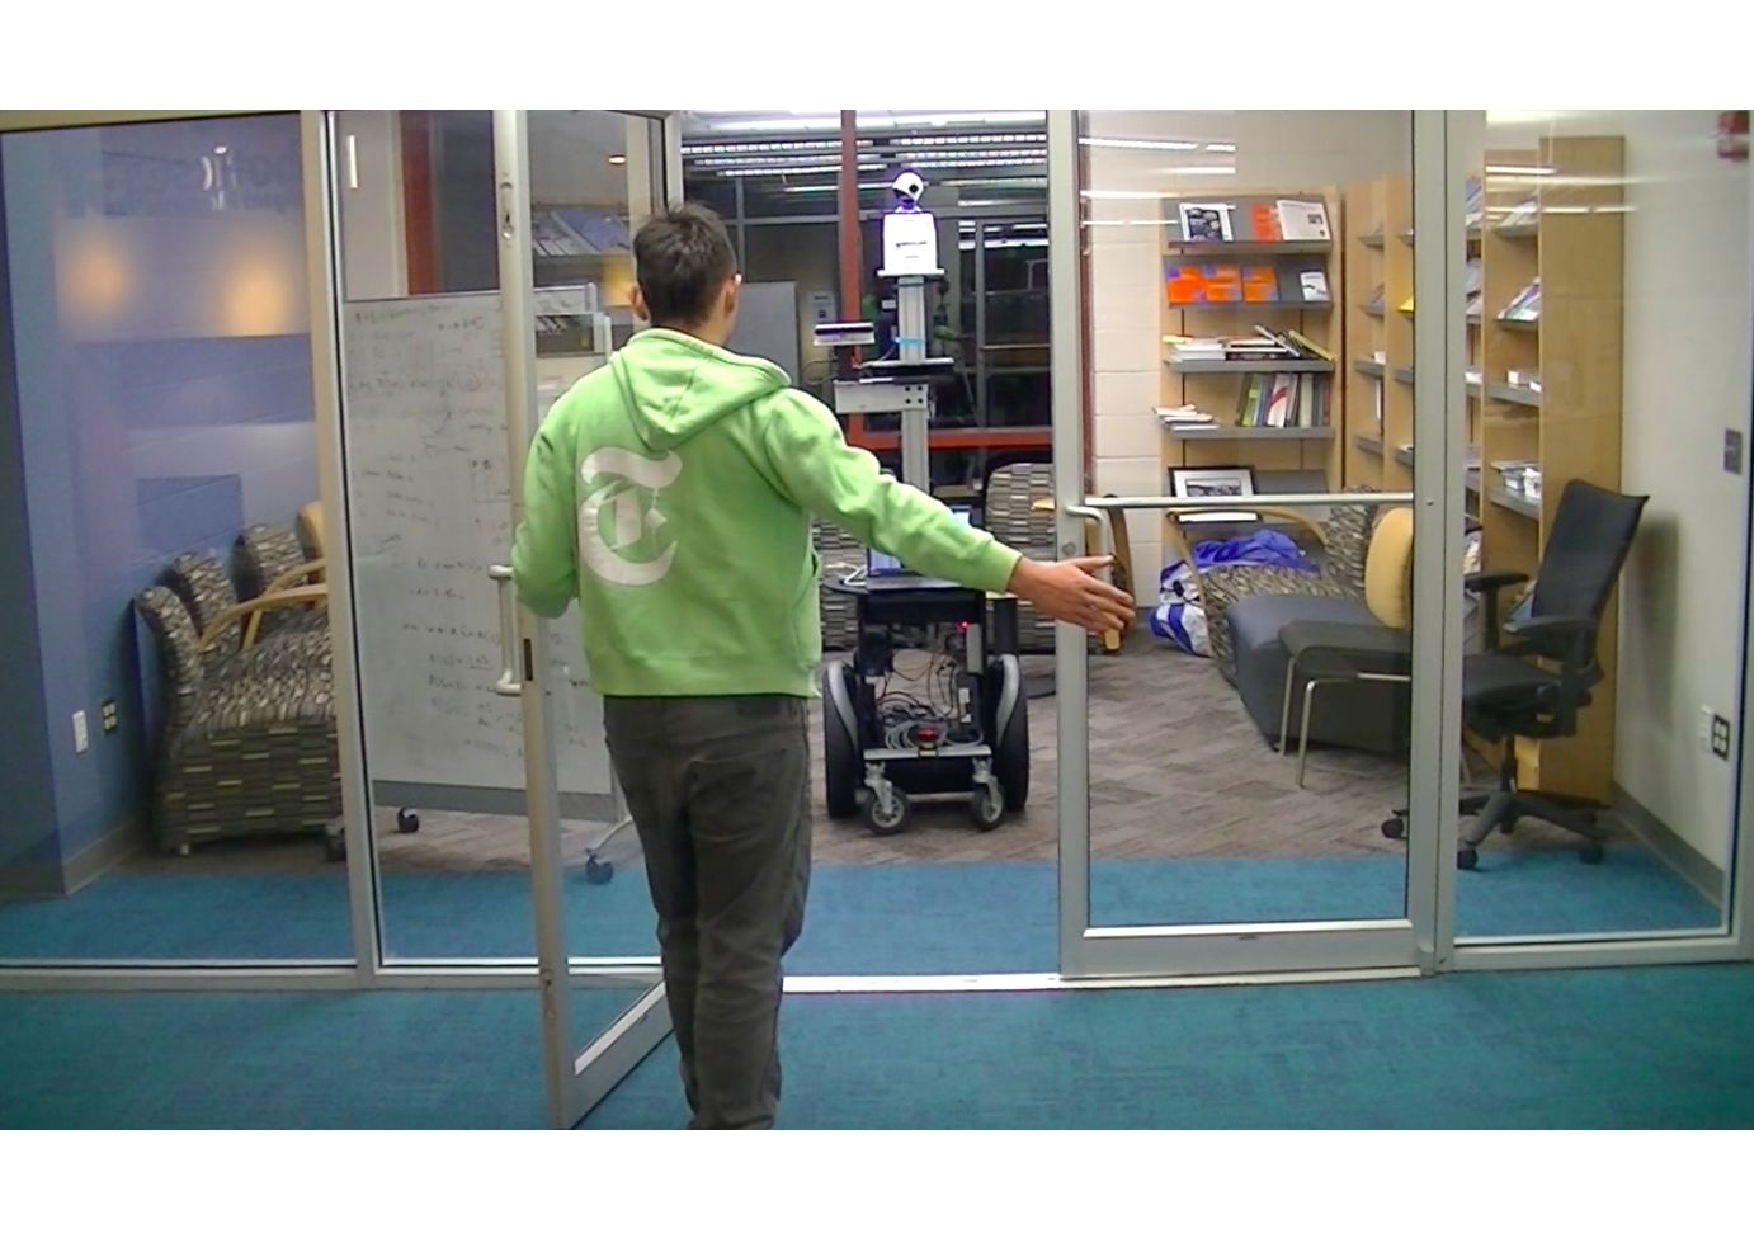
\includegraphics[width=0.45\textwidth]{pics/sit_door_01}
        } \\
        \subfigure[]{%
        	\label{fig:situtation_aware_door_passing2}
            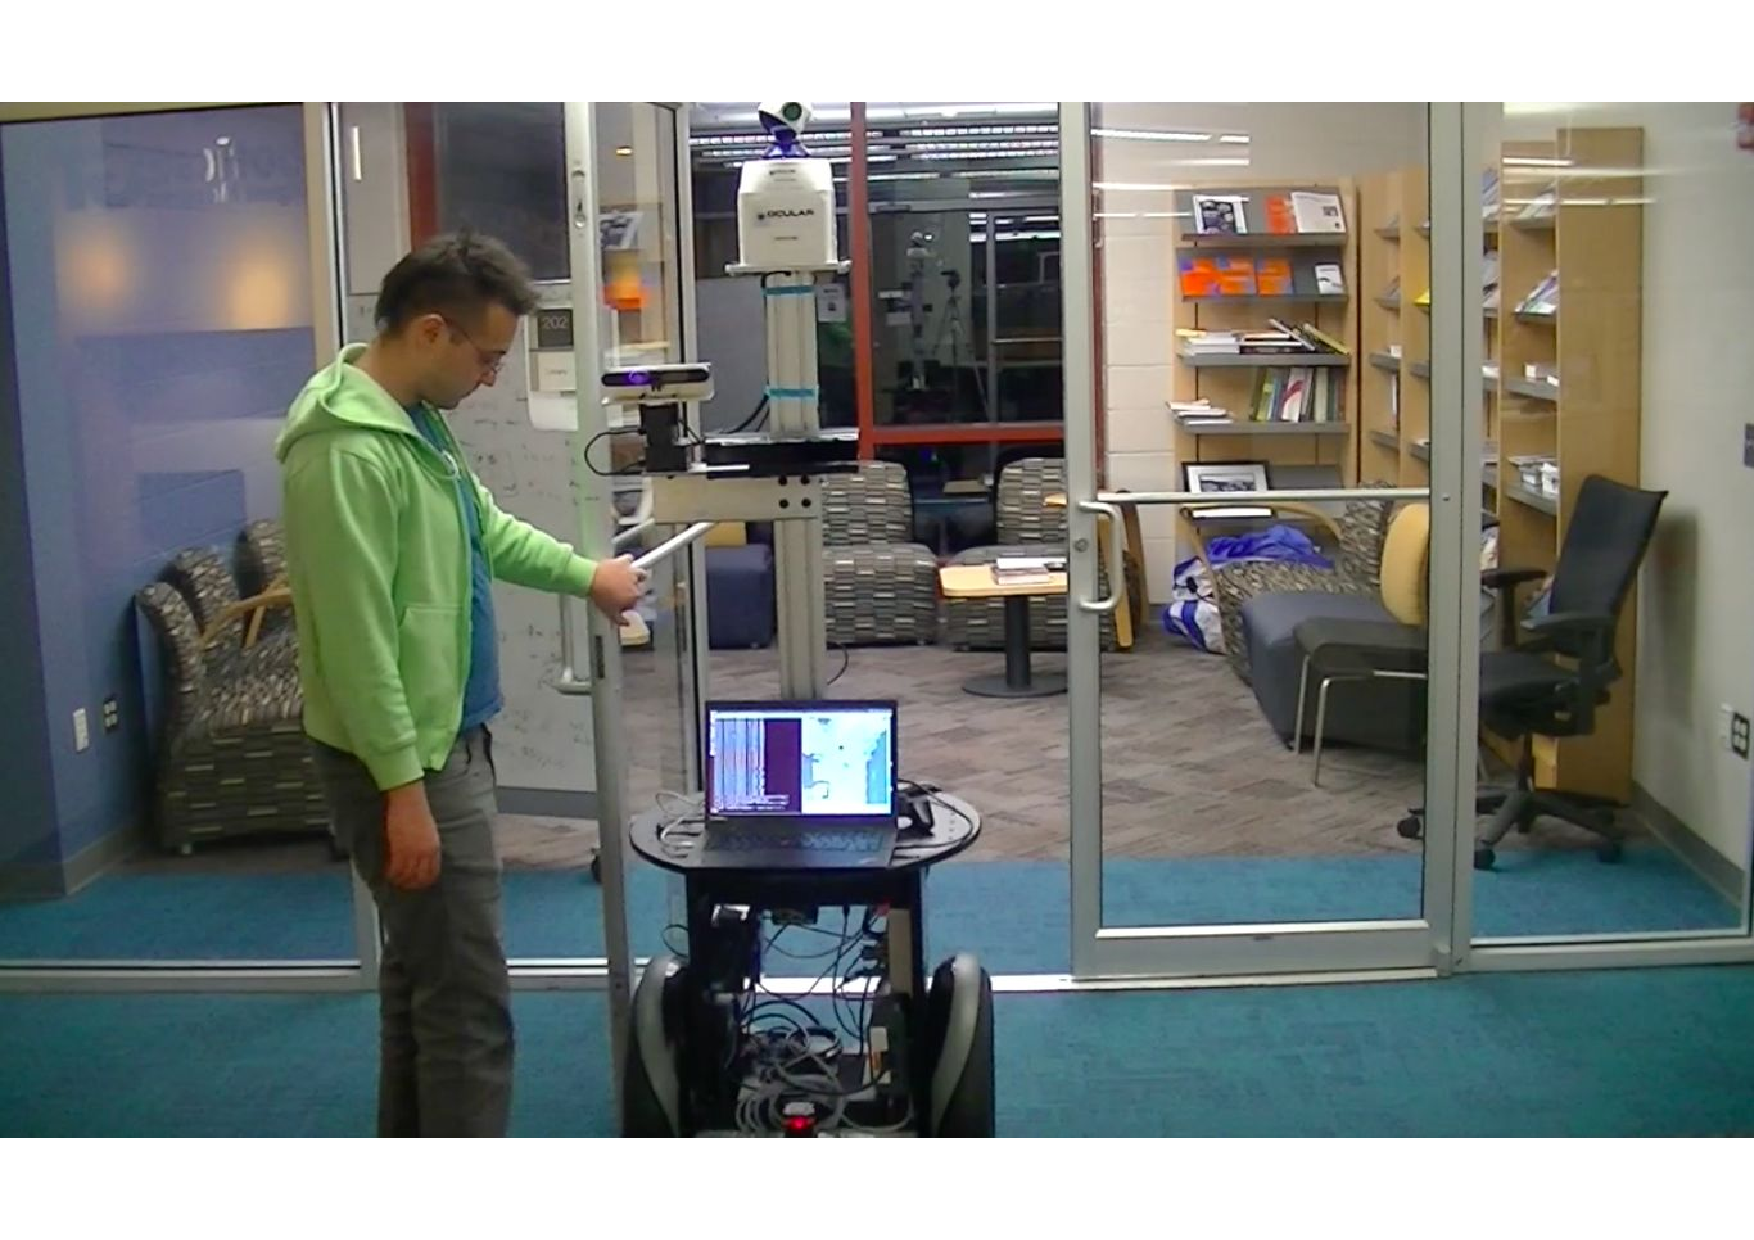
\includegraphics[width=0.45\textwidth]{pics/sit_door_03}
        }%\\        
        \subfigure[]{%           
           \label{fig:situtation_aware_door_passing3}
           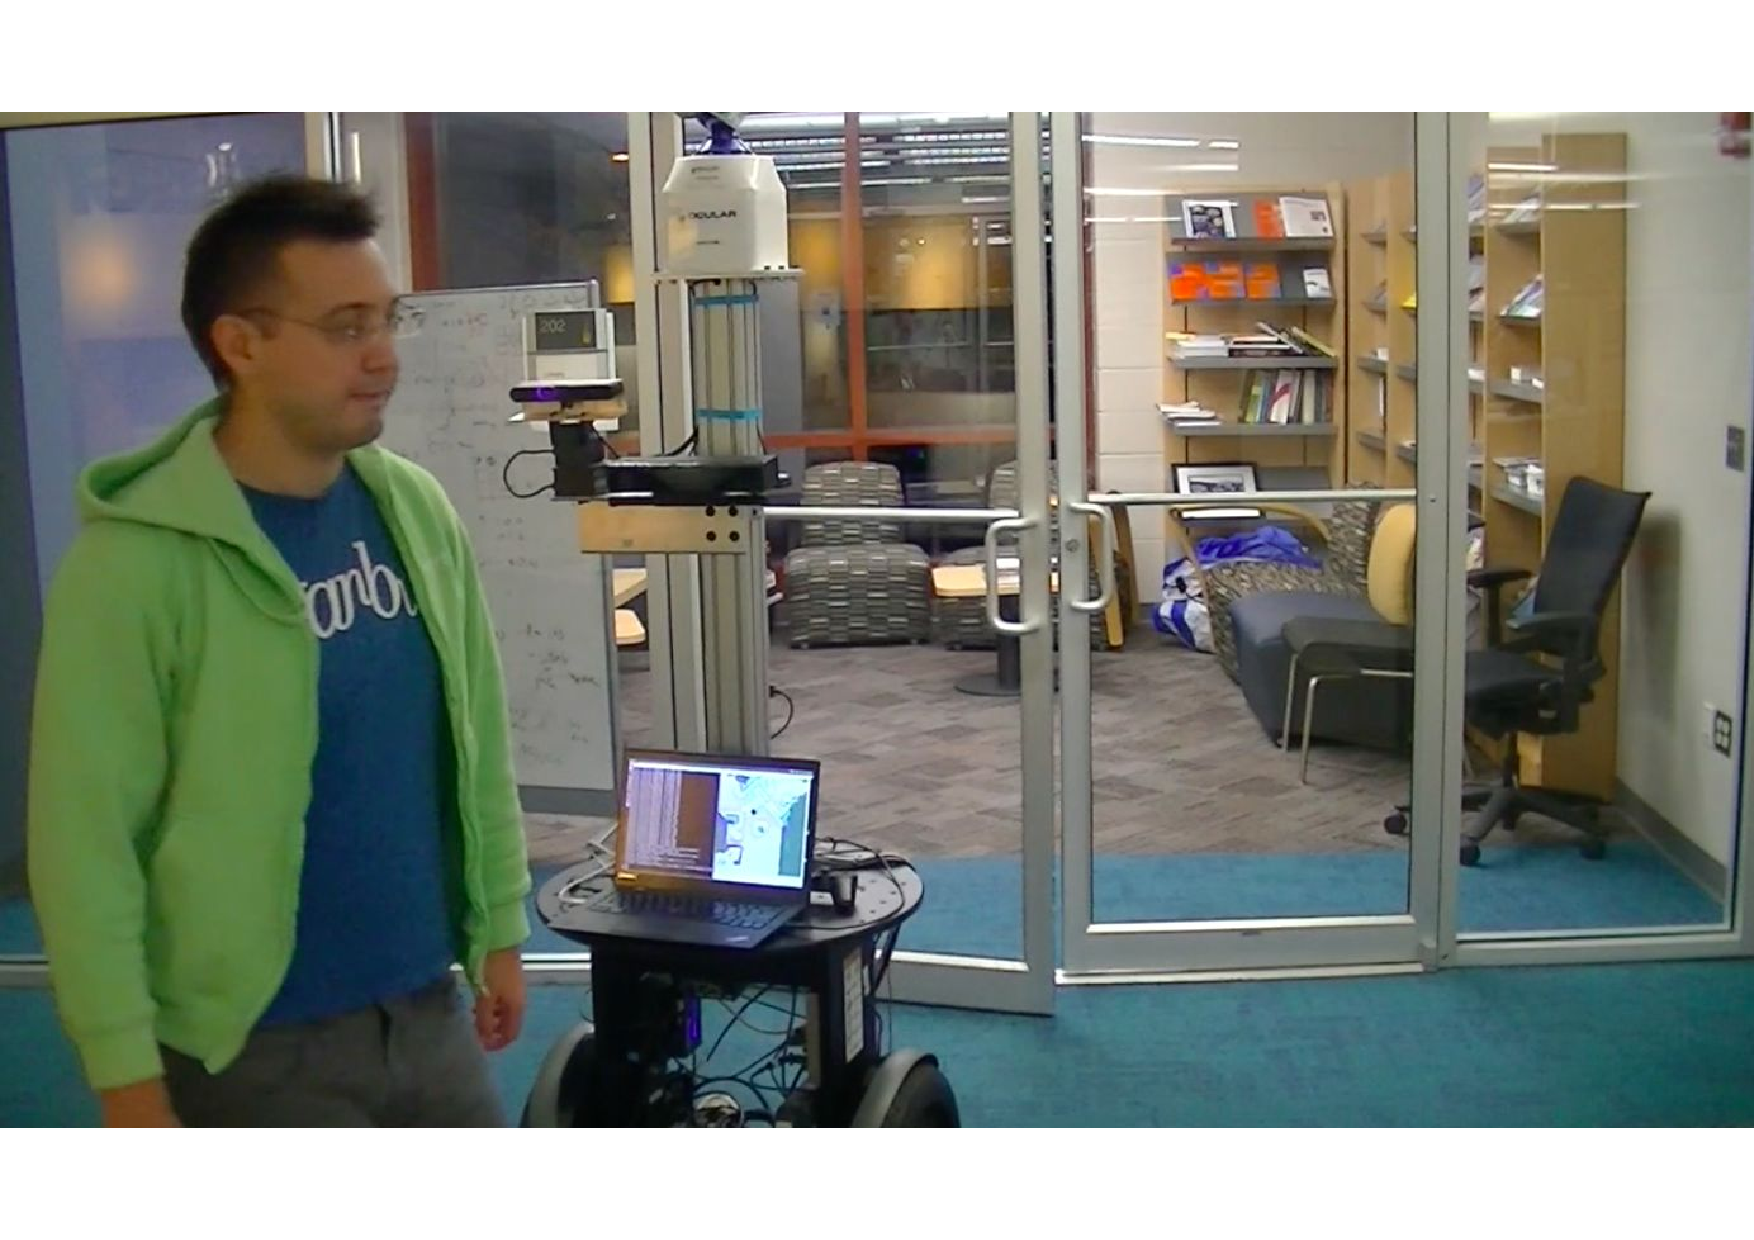
\includegraphics[width=0.46\textwidth]{pics/sit_door_04}
        }
    \caption{Demonstration of context-awareness for door passing during person following. This is a swing door with spring loaded hinges, so it would close if not kept open actively. a) The robot is following the user by keeping a fixed distance to the user. b) Signal phase: The user has stopped, is in close proximity to the door and performed a pointing gesture toward the other room. c) Approach Phase: The robot passes the door while the user is holding the door d) Release Phase: User has more than a threshold distance to the door, and robot continues with the basic following.}
   \label{fig:situtation_aware_door_passing}
\end{figure}



\section{Conclusion}
\label{sec:conclusions}

In this paper, we discussed the process of building semantic maps, how to interactively label entities in it, and use them to enable new navigation behaviors for specific scenarios. We utilize planar surfaces such as walls and tables, and static objects such as door signs as features to our semantic SLAM approach. Users can interactively annotate these features by having the robot follow him/her, entering the label through a mobile app and performing a pointing gesture toward the landmark of interest. These landmarks can later be used to generate context-aware motions.

Our pointing gesture approach can reliably estimate the target object using human joint positions and detect ambiguous gestures with probabilistic modeling. Our person following algorithm attempts to maximize future utility by searching future actions, assuming constant velocity model for the human. We showed that our person following method can keep a near-constant distance to the human. We described a simple method to extract metric goals from a semantic map landmark and presented a human-aware path planner that considers the personal spaces of people to generate socially-aware paths. Finally, we demonstrated context-awareness for person following in two scenarios: interactive labeling and door passing. For interactive labeling, the robot utilizes the task knowledge and moves to a favorable position to facilitate interaction if an unlabeled landmark is detected near the person. For door passing, the robot utilizes the existence of a door passage, by querying detected door signs in the semantic map, to enter a door passage behavior.

Semantic maps would facilitate communication of goals from a HRI perspective and enable navigation behaviors that are not feasible with metric maps. We showed proof of concept for enabling context-aware navigation behaviors using semantics and believe that there is much to explore in this research area. We think as the sensing technology improves and maps with richer semantic information becomes common, it would make intelligent navigation algorithms possible.

One limitation of our work is that there is only implicit interaction between the robot and human in our interaction design. The robot signaled its intention only through motion and did not explicitly communicate with people. As future work, dialogue and gaze could be utilized to complement the motions of the robot. We also plan to evaluate the effectiveness of context-awareness navigation with user studies.

\bibliographystyle{tADR}
\bibliography{semantic_maps}


\end{document}
